% Created by tikzDevice version 0.12.6 on 2025-02-16 19:11:30
% !TEX encoding = UTF-8 Unicode
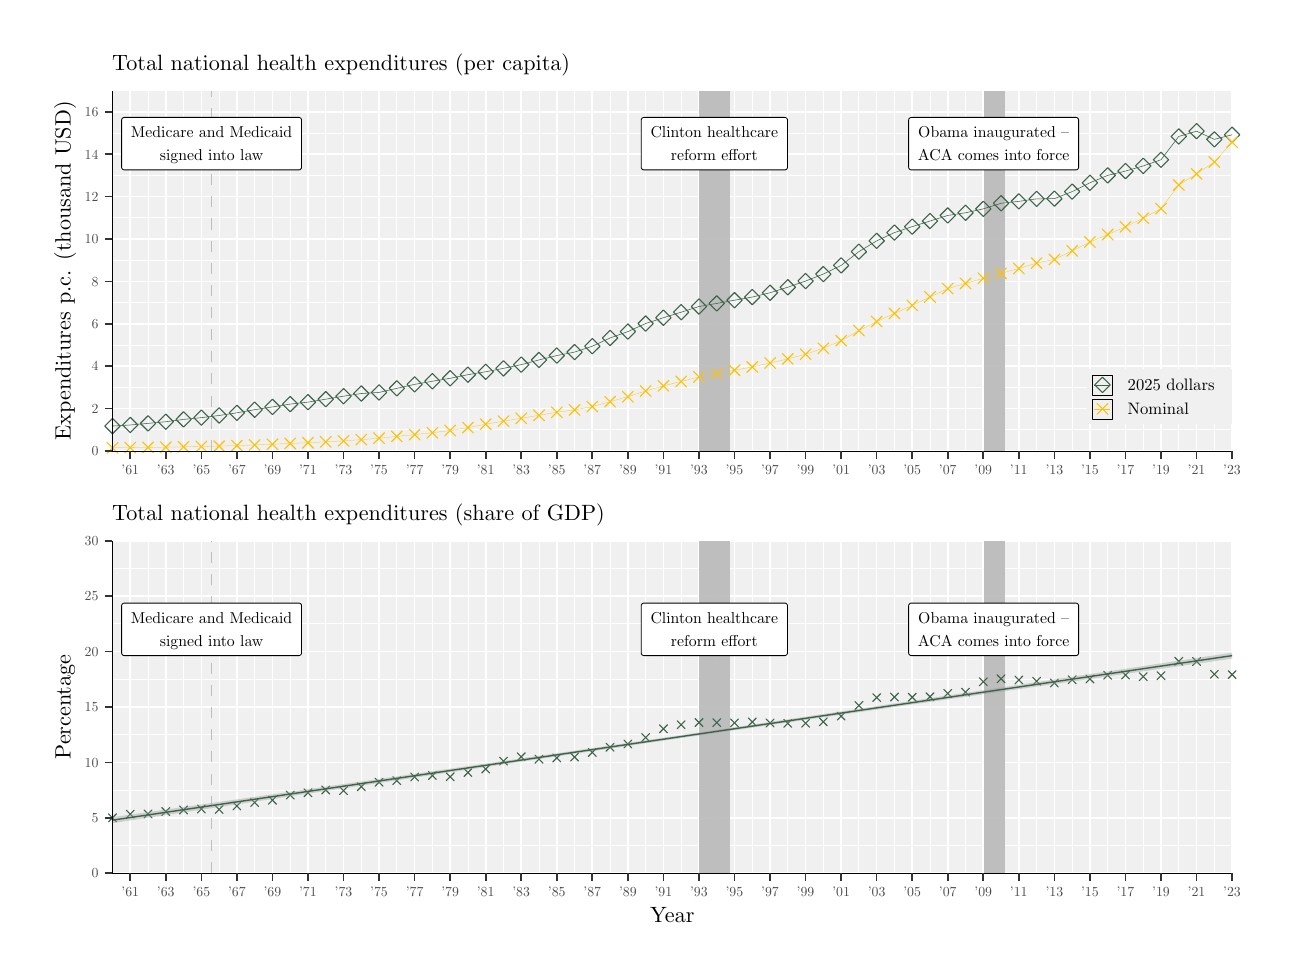
\begin{tikzpicture}[x=1pt,y=1pt]
\definecolor{fillColor}{RGB}{255,255,255}
\path[use as bounding box,fill=fillColor,fill opacity=0.00] (0,0) rectangle (455.30,325.21);
\begin{scope}
\path[clip] (  0.00,162.61) rectangle (455.30,325.21);
\definecolor{drawColor}{RGB}{255,255,255}
\definecolor{fillColor}{RGB}{255,255,255}

\path[draw=drawColor,line width= 0.6pt,line join=round,line cap=round,fill=fillColor] (  0.00,162.61) rectangle (455.30,325.21);
\end{scope}
\begin{scope}
\path[clip] (  0.00,  0.00) rectangle (455.30,325.21);
\definecolor{fillColor}{gray}{0.94}

\path[fill=fillColor] ( 30.56,172.27) rectangle (435.30,302.44);
\definecolor{drawColor}{RGB}{255,255,255}

\path[draw=drawColor,line width= 0.3pt,line join=round] ( 30.56,179.92) --
	(435.30,179.92);

\path[draw=drawColor,line width= 0.3pt,line join=round] ( 30.56,195.24) --
	(435.30,195.24);

\path[draw=drawColor,line width= 0.3pt,line join=round] ( 30.56,210.55) --
	(435.30,210.55);

\path[draw=drawColor,line width= 0.3pt,line join=round] ( 30.56,225.87) --
	(435.30,225.87);

\path[draw=drawColor,line width= 0.3pt,line join=round] ( 30.56,241.18) --
	(435.30,241.18);

\path[draw=drawColor,line width= 0.3pt,line join=round] ( 30.56,256.50) --
	(435.30,256.50);

\path[draw=drawColor,line width= 0.3pt,line join=round] ( 30.56,271.81) --
	(435.30,271.81);

\path[draw=drawColor,line width= 0.3pt,line join=round] ( 30.56,287.12) --
	(435.30,287.12);

\path[draw=drawColor,line width= 0.3pt,line join=round] ( 30.56,302.44) --
	(435.30,302.44);

\path[draw=drawColor,line width= 0.3pt,line join=round] ( 30.65,172.27) --
	( 30.65,302.44);

\path[draw=drawColor,line width= 0.3pt,line join=round] ( 43.50,172.27) --
	( 43.50,302.44);

\path[draw=drawColor,line width= 0.3pt,line join=round] ( 56.34,172.27) --
	( 56.34,302.44);

\path[draw=drawColor,line width= 0.3pt,line join=round] ( 69.18,172.27) --
	( 69.18,302.44);

\path[draw=drawColor,line width= 0.3pt,line join=round] ( 82.03,172.27) --
	( 82.03,302.44);

\path[draw=drawColor,line width= 0.3pt,line join=round] ( 94.87,172.27) --
	( 94.87,302.44);

\path[draw=drawColor,line width= 0.3pt,line join=round] (107.71,172.27) --
	(107.71,302.44);

\path[draw=drawColor,line width= 0.3pt,line join=round] (120.56,172.27) --
	(120.56,302.44);

\path[draw=drawColor,line width= 0.3pt,line join=round] (133.40,172.27) --
	(133.40,302.44);

\path[draw=drawColor,line width= 0.3pt,line join=round] (146.24,172.27) --
	(146.24,302.44);

\path[draw=drawColor,line width= 0.3pt,line join=round] (159.09,172.27) --
	(159.09,302.44);

\path[draw=drawColor,line width= 0.3pt,line join=round] (171.93,172.27) --
	(171.93,302.44);

\path[draw=drawColor,line width= 0.3pt,line join=round] (184.77,172.27) --
	(184.77,302.44);

\path[draw=drawColor,line width= 0.3pt,line join=round] (197.62,172.27) --
	(197.62,302.44);

\path[draw=drawColor,line width= 0.3pt,line join=round] (210.46,172.27) --
	(210.46,302.44);

\path[draw=drawColor,line width= 0.3pt,line join=round] (223.30,172.27) --
	(223.30,302.44);

\path[draw=drawColor,line width= 0.3pt,line join=round] (236.15,172.27) --
	(236.15,302.44);

\path[draw=drawColor,line width= 0.3pt,line join=round] (248.99,172.27) --
	(248.99,302.44);

\path[draw=drawColor,line width= 0.3pt,line join=round] (261.83,172.27) --
	(261.83,302.44);

\path[draw=drawColor,line width= 0.3pt,line join=round] (274.68,172.27) --
	(274.68,302.44);

\path[draw=drawColor,line width= 0.3pt,line join=round] (287.52,172.27) --
	(287.52,302.44);

\path[draw=drawColor,line width= 0.3pt,line join=round] (300.36,172.27) --
	(300.36,302.44);

\path[draw=drawColor,line width= 0.3pt,line join=round] (313.21,172.27) --
	(313.21,302.44);

\path[draw=drawColor,line width= 0.3pt,line join=round] (326.05,172.27) --
	(326.05,302.44);

\path[draw=drawColor,line width= 0.3pt,line join=round] (338.89,172.27) --
	(338.89,302.44);

\path[draw=drawColor,line width= 0.3pt,line join=round] (351.74,172.27) --
	(351.74,302.44);

\path[draw=drawColor,line width= 0.3pt,line join=round] (364.58,172.27) --
	(364.58,302.44);

\path[draw=drawColor,line width= 0.3pt,line join=round] (377.42,172.27) --
	(377.42,302.44);

\path[draw=drawColor,line width= 0.3pt,line join=round] (390.27,172.27) --
	(390.27,302.44);

\path[draw=drawColor,line width= 0.3pt,line join=round] (403.11,172.27) --
	(403.11,302.44);

\path[draw=drawColor,line width= 0.3pt,line join=round] (415.95,172.27) --
	(415.95,302.44);

\path[draw=drawColor,line width= 0.3pt,line join=round] (428.80,172.27) --
	(428.80,302.44);

\path[draw=drawColor,line width= 0.6pt,line join=round] ( 30.56,172.27) --
	(435.30,172.27);

\path[draw=drawColor,line width= 0.6pt,line join=round] ( 30.56,187.58) --
	(435.30,187.58);

\path[draw=drawColor,line width= 0.6pt,line join=round] ( 30.56,202.89) --
	(435.30,202.89);

\path[draw=drawColor,line width= 0.6pt,line join=round] ( 30.56,218.21) --
	(435.30,218.21);

\path[draw=drawColor,line width= 0.6pt,line join=round] ( 30.56,233.52) --
	(435.30,233.52);

\path[draw=drawColor,line width= 0.6pt,line join=round] ( 30.56,248.84) --
	(435.30,248.84);

\path[draw=drawColor,line width= 0.6pt,line join=round] ( 30.56,264.15) --
	(435.30,264.15);

\path[draw=drawColor,line width= 0.6pt,line join=round] ( 30.56,279.47) --
	(435.30,279.47);

\path[draw=drawColor,line width= 0.6pt,line join=round] ( 30.56,294.78) --
	(435.30,294.78);

\path[draw=drawColor,line width= 0.6pt,line join=round] ( 37.08,172.27) --
	( 37.08,302.44);

\path[draw=drawColor,line width= 0.6pt,line join=round] ( 49.91,172.27) --
	( 49.91,302.44);

\path[draw=drawColor,line width= 0.6pt,line join=round] ( 62.77,172.27) --
	( 62.77,302.44);

\path[draw=drawColor,line width= 0.6pt,line join=round] ( 75.60,172.27) --
	( 75.60,302.44);

\path[draw=drawColor,line width= 0.6pt,line join=round] ( 88.45,172.27) --
	( 88.45,302.44);

\path[draw=drawColor,line width= 0.6pt,line join=round] (101.29,172.27) --
	(101.29,302.44);

\path[draw=drawColor,line width= 0.6pt,line join=round] (114.14,172.27) --
	(114.14,302.44);

\path[draw=drawColor,line width= 0.6pt,line join=round] (126.97,172.27) --
	(126.97,302.44);

\path[draw=drawColor,line width= 0.6pt,line join=round] (139.83,172.27) --
	(139.83,302.44);

\path[draw=drawColor,line width= 0.6pt,line join=round] (152.66,172.27) --
	(152.66,302.44);

\path[draw=drawColor,line width= 0.6pt,line join=round] (165.51,172.27) --
	(165.51,302.44);

\path[draw=drawColor,line width= 0.6pt,line join=round] (178.35,172.27) --
	(178.35,302.44);

\path[draw=drawColor,line width= 0.6pt,line join=round] (191.20,172.27) --
	(191.20,302.44);

\path[draw=drawColor,line width= 0.6pt,line join=round] (204.03,172.27) --
	(204.03,302.44);

\path[draw=drawColor,line width= 0.6pt,line join=round] (216.89,172.27) --
	(216.89,302.44);

\path[draw=drawColor,line width= 0.6pt,line join=round] (229.72,172.27) --
	(229.72,302.44);

\path[draw=drawColor,line width= 0.6pt,line join=round] (242.57,172.27) --
	(242.57,302.44);

\path[draw=drawColor,line width= 0.6pt,line join=round] (255.41,172.27) --
	(255.41,302.44);

\path[draw=drawColor,line width= 0.6pt,line join=round] (268.26,172.27) --
	(268.26,302.44);

\path[draw=drawColor,line width= 0.6pt,line join=round] (281.09,172.27) --
	(281.09,302.44);

\path[draw=drawColor,line width= 0.6pt,line join=round] (293.95,172.27) --
	(293.95,302.44);

\path[draw=drawColor,line width= 0.6pt,line join=round] (306.78,172.27) --
	(306.78,302.44);

\path[draw=drawColor,line width= 0.6pt,line join=round] (319.63,172.27) --
	(319.63,302.44);

\path[draw=drawColor,line width= 0.6pt,line join=round] (332.47,172.27) --
	(332.47,302.44);

\path[draw=drawColor,line width= 0.6pt,line join=round] (345.32,172.27) --
	(345.32,302.44);

\path[draw=drawColor,line width= 0.6pt,line join=round] (358.15,172.27) --
	(358.15,302.44);

\path[draw=drawColor,line width= 0.6pt,line join=round] (371.01,172.27) --
	(371.01,302.44);

\path[draw=drawColor,line width= 0.6pt,line join=round] (383.84,172.27) --
	(383.84,302.44);

\path[draw=drawColor,line width= 0.6pt,line join=round] (396.69,172.27) --
	(396.69,302.44);

\path[draw=drawColor,line width= 0.6pt,line join=round] (409.53,172.27) --
	(409.53,302.44);

\path[draw=drawColor,line width= 0.6pt,line join=round] (422.38,172.27) --
	(422.38,302.44);

\path[draw=drawColor,line width= 0.6pt,line join=round] (435.21,172.27) --
	(435.21,302.44);
\definecolor{drawColor}{RGB}{190,190,190}

\path[draw=drawColor,line width= 0.6pt,line join=round] ( 30.65,172.27) -- ( 30.65,302.44);
\definecolor{fillColor}{RGB}{190,190,190}

\path[fill=fillColor,fill opacity=0.01] (242.57,172.27) rectangle (253.70,302.44);

\path[fill=fillColor,fill opacity=0.01] (242.57,172.27) rectangle (253.70,302.44);

\path[fill=fillColor,fill opacity=0.01] (242.57,172.27) rectangle (253.70,302.44);

\path[fill=fillColor,fill opacity=0.01] (242.57,172.27) rectangle (253.70,302.44);

\path[fill=fillColor,fill opacity=0.01] (242.57,172.27) rectangle (253.70,302.44);

\path[fill=fillColor,fill opacity=0.01] (242.57,172.27) rectangle (253.70,302.44);

\path[fill=fillColor,fill opacity=0.01] (242.57,172.27) rectangle (253.70,302.44);

\path[fill=fillColor,fill opacity=0.01] (242.57,172.27) rectangle (253.70,302.44);

\path[fill=fillColor,fill opacity=0.01] (242.57,172.27) rectangle (253.70,302.44);

\path[fill=fillColor,fill opacity=0.01] (242.57,172.27) rectangle (253.70,302.44);

\path[fill=fillColor,fill opacity=0.01] (242.57,172.27) rectangle (253.70,302.44);

\path[fill=fillColor,fill opacity=0.01] (242.57,172.27) rectangle (253.70,302.44);

\path[fill=fillColor,fill opacity=0.01] (242.57,172.27) rectangle (253.70,302.44);

\path[fill=fillColor,fill opacity=0.01] (242.57,172.27) rectangle (253.70,302.44);

\path[fill=fillColor,fill opacity=0.01] (242.57,172.27) rectangle (253.70,302.44);

\path[fill=fillColor,fill opacity=0.01] (242.57,172.27) rectangle (253.70,302.44);

\path[fill=fillColor,fill opacity=0.01] (242.57,172.27) rectangle (253.70,302.44);

\path[fill=fillColor,fill opacity=0.01] (242.57,172.27) rectangle (253.70,302.44);

\path[fill=fillColor,fill opacity=0.01] (242.57,172.27) rectangle (253.70,302.44);

\path[fill=fillColor,fill opacity=0.01] (242.57,172.27) rectangle (253.70,302.44);

\path[fill=fillColor,fill opacity=0.01] (242.57,172.27) rectangle (253.70,302.44);

\path[fill=fillColor,fill opacity=0.01] (242.57,172.27) rectangle (253.70,302.44);

\path[fill=fillColor,fill opacity=0.01] (242.57,172.27) rectangle (253.70,302.44);

\path[fill=fillColor,fill opacity=0.01] (242.57,172.27) rectangle (253.70,302.44);

\path[fill=fillColor,fill opacity=0.01] (242.57,172.27) rectangle (253.70,302.44);

\path[fill=fillColor,fill opacity=0.01] (242.57,172.27) rectangle (253.70,302.44);

\path[fill=fillColor,fill opacity=0.01] (242.57,172.27) rectangle (253.70,302.44);

\path[fill=fillColor,fill opacity=0.01] (242.57,172.27) rectangle (253.70,302.44);

\path[fill=fillColor,fill opacity=0.01] (242.57,172.27) rectangle (253.70,302.44);

\path[fill=fillColor,fill opacity=0.01] (242.57,172.27) rectangle (253.70,302.44);

\path[fill=fillColor,fill opacity=0.01] (242.57,172.27) rectangle (253.70,302.44);

\path[fill=fillColor,fill opacity=0.01] (242.57,172.27) rectangle (253.70,302.44);

\path[fill=fillColor,fill opacity=0.01] (242.57,172.27) rectangle (253.70,302.44);

\path[fill=fillColor,fill opacity=0.01] (242.57,172.27) rectangle (253.70,302.44);

\path[fill=fillColor,fill opacity=0.01] (242.57,172.27) rectangle (253.70,302.44);

\path[fill=fillColor,fill opacity=0.01] (242.57,172.27) rectangle (253.70,302.44);

\path[fill=fillColor,fill opacity=0.01] (242.57,172.27) rectangle (253.70,302.44);

\path[fill=fillColor,fill opacity=0.01] (242.57,172.27) rectangle (253.70,302.44);

\path[fill=fillColor,fill opacity=0.01] (242.57,172.27) rectangle (253.70,302.44);

\path[fill=fillColor,fill opacity=0.01] (242.57,172.27) rectangle (253.70,302.44);

\path[fill=fillColor,fill opacity=0.01] (242.57,172.27) rectangle (253.70,302.44);

\path[fill=fillColor,fill opacity=0.01] (242.57,172.27) rectangle (253.70,302.44);

\path[fill=fillColor,fill opacity=0.01] (242.57,172.27) rectangle (253.70,302.44);

\path[fill=fillColor,fill opacity=0.01] (242.57,172.27) rectangle (253.70,302.44);

\path[fill=fillColor,fill opacity=0.01] (242.57,172.27) rectangle (253.70,302.44);

\path[fill=fillColor,fill opacity=0.01] (242.57,172.27) rectangle (253.70,302.44);

\path[fill=fillColor,fill opacity=0.01] (242.57,172.27) rectangle (253.70,302.44);

\path[fill=fillColor,fill opacity=0.01] (242.57,172.27) rectangle (253.70,302.44);

\path[fill=fillColor,fill opacity=0.01] (242.57,172.27) rectangle (253.70,302.44);

\path[fill=fillColor,fill opacity=0.01] (242.57,172.27) rectangle (253.70,302.44);

\path[fill=fillColor,fill opacity=0.01] (242.57,172.27) rectangle (253.70,302.44);

\path[fill=fillColor,fill opacity=0.01] (242.57,172.27) rectangle (253.70,302.44);

\path[fill=fillColor,fill opacity=0.01] (242.57,172.27) rectangle (253.70,302.44);

\path[fill=fillColor,fill opacity=0.01] (242.57,172.27) rectangle (253.70,302.44);

\path[fill=fillColor,fill opacity=0.01] (242.57,172.27) rectangle (253.70,302.44);

\path[fill=fillColor,fill opacity=0.01] (242.57,172.27) rectangle (253.70,302.44);

\path[fill=fillColor,fill opacity=0.01] (242.57,172.27) rectangle (253.70,302.44);

\path[fill=fillColor,fill opacity=0.01] (242.57,172.27) rectangle (253.70,302.44);

\path[fill=fillColor,fill opacity=0.01] (242.57,172.27) rectangle (253.70,302.44);

\path[fill=fillColor,fill opacity=0.01] (242.57,172.27) rectangle (253.70,302.44);

\path[fill=fillColor,fill opacity=0.01] (242.57,172.27) rectangle (253.70,302.44);

\path[fill=fillColor,fill opacity=0.01] (242.57,172.27) rectangle (253.70,302.44);

\path[fill=fillColor,fill opacity=0.01] (242.57,172.27) rectangle (253.70,302.44);

\path[fill=fillColor,fill opacity=0.01] (242.57,172.27) rectangle (253.70,302.44);

\path[fill=fillColor,fill opacity=0.01] (345.65,172.27) rectangle (353.16,302.44);

\path[fill=fillColor,fill opacity=0.01] (345.65,172.27) rectangle (353.16,302.44);

\path[fill=fillColor,fill opacity=0.01] (345.65,172.27) rectangle (353.16,302.44);

\path[fill=fillColor,fill opacity=0.01] (345.65,172.27) rectangle (353.16,302.44);

\path[fill=fillColor,fill opacity=0.01] (345.65,172.27) rectangle (353.16,302.44);

\path[fill=fillColor,fill opacity=0.01] (345.65,172.27) rectangle (353.16,302.44);

\path[fill=fillColor,fill opacity=0.01] (345.65,172.27) rectangle (353.16,302.44);

\path[fill=fillColor,fill opacity=0.01] (345.65,172.27) rectangle (353.16,302.44);

\path[fill=fillColor,fill opacity=0.01] (345.65,172.27) rectangle (353.16,302.44);

\path[fill=fillColor,fill opacity=0.01] (345.65,172.27) rectangle (353.16,302.44);

\path[fill=fillColor,fill opacity=0.01] (345.65,172.27) rectangle (353.16,302.44);

\path[fill=fillColor,fill opacity=0.01] (345.65,172.27) rectangle (353.16,302.44);

\path[fill=fillColor,fill opacity=0.01] (345.65,172.27) rectangle (353.16,302.44);

\path[fill=fillColor,fill opacity=0.01] (345.65,172.27) rectangle (353.16,302.44);

\path[fill=fillColor,fill opacity=0.01] (345.65,172.27) rectangle (353.16,302.44);

\path[fill=fillColor,fill opacity=0.01] (345.65,172.27) rectangle (353.16,302.44);

\path[fill=fillColor,fill opacity=0.01] (345.65,172.27) rectangle (353.16,302.44);

\path[fill=fillColor,fill opacity=0.01] (345.65,172.27) rectangle (353.16,302.44);

\path[fill=fillColor,fill opacity=0.01] (345.65,172.27) rectangle (353.16,302.44);

\path[fill=fillColor,fill opacity=0.01] (345.65,172.27) rectangle (353.16,302.44);

\path[fill=fillColor,fill opacity=0.01] (345.65,172.27) rectangle (353.16,302.44);

\path[fill=fillColor,fill opacity=0.01] (345.65,172.27) rectangle (353.16,302.44);

\path[fill=fillColor,fill opacity=0.01] (345.65,172.27) rectangle (353.16,302.44);

\path[fill=fillColor,fill opacity=0.01] (345.65,172.27) rectangle (353.16,302.44);

\path[fill=fillColor,fill opacity=0.01] (345.65,172.27) rectangle (353.16,302.44);

\path[fill=fillColor,fill opacity=0.01] (345.65,172.27) rectangle (353.16,302.44);

\path[fill=fillColor,fill opacity=0.01] (345.65,172.27) rectangle (353.16,302.44);

\path[fill=fillColor,fill opacity=0.01] (345.65,172.27) rectangle (353.16,302.44);

\path[fill=fillColor,fill opacity=0.01] (345.65,172.27) rectangle (353.16,302.44);

\path[fill=fillColor,fill opacity=0.01] (345.65,172.27) rectangle (353.16,302.44);

\path[fill=fillColor,fill opacity=0.01] (345.65,172.27) rectangle (353.16,302.44);

\path[fill=fillColor,fill opacity=0.01] (345.65,172.27) rectangle (353.16,302.44);

\path[fill=fillColor,fill opacity=0.01] (345.65,172.27) rectangle (353.16,302.44);

\path[fill=fillColor,fill opacity=0.01] (345.65,172.27) rectangle (353.16,302.44);

\path[fill=fillColor,fill opacity=0.01] (345.65,172.27) rectangle (353.16,302.44);

\path[fill=fillColor,fill opacity=0.01] (345.65,172.27) rectangle (353.16,302.44);

\path[fill=fillColor,fill opacity=0.01] (345.65,172.27) rectangle (353.16,302.44);

\path[fill=fillColor,fill opacity=0.01] (345.65,172.27) rectangle (353.16,302.44);

\path[fill=fillColor,fill opacity=0.01] (345.65,172.27) rectangle (353.16,302.44);

\path[fill=fillColor,fill opacity=0.01] (345.65,172.27) rectangle (353.16,302.44);

\path[fill=fillColor,fill opacity=0.01] (345.65,172.27) rectangle (353.16,302.44);

\path[fill=fillColor,fill opacity=0.01] (345.65,172.27) rectangle (353.16,302.44);

\path[fill=fillColor,fill opacity=0.01] (345.65,172.27) rectangle (353.16,302.44);

\path[fill=fillColor,fill opacity=0.01] (345.65,172.27) rectangle (353.16,302.44);

\path[fill=fillColor,fill opacity=0.01] (345.65,172.27) rectangle (353.16,302.44);

\path[fill=fillColor,fill opacity=0.01] (345.65,172.27) rectangle (353.16,302.44);

\path[fill=fillColor,fill opacity=0.01] (345.65,172.27) rectangle (353.16,302.44);

\path[fill=fillColor,fill opacity=0.01] (345.65,172.27) rectangle (353.16,302.44);

\path[fill=fillColor,fill opacity=0.01] (345.65,172.27) rectangle (353.16,302.44);

\path[fill=fillColor,fill opacity=0.01] (345.65,172.27) rectangle (353.16,302.44);

\path[fill=fillColor,fill opacity=0.01] (345.65,172.27) rectangle (353.16,302.44);

\path[fill=fillColor,fill opacity=0.01] (345.65,172.27) rectangle (353.16,302.44);

\path[fill=fillColor,fill opacity=0.01] (345.65,172.27) rectangle (353.16,302.44);

\path[fill=fillColor,fill opacity=0.01] (345.65,172.27) rectangle (353.16,302.44);

\path[fill=fillColor,fill opacity=0.01] (345.65,172.27) rectangle (353.16,302.44);

\path[fill=fillColor,fill opacity=0.01] (345.65,172.27) rectangle (353.16,302.44);

\path[fill=fillColor,fill opacity=0.01] (345.65,172.27) rectangle (353.16,302.44);

\path[fill=fillColor,fill opacity=0.01] (345.65,172.27) rectangle (353.16,302.44);

\path[fill=fillColor,fill opacity=0.01] (345.65,172.27) rectangle (353.16,302.44);

\path[fill=fillColor,fill opacity=0.01] (345.65,172.27) rectangle (353.16,302.44);

\path[fill=fillColor,fill opacity=0.01] (345.65,172.27) rectangle (353.16,302.44);

\path[fill=fillColor,fill opacity=0.01] (345.65,172.27) rectangle (353.16,302.44);

\path[fill=fillColor,fill opacity=0.01] (345.65,172.27) rectangle (353.16,302.44);

\path[fill=fillColor,fill opacity=0.01] (345.65,172.27) rectangle (353.16,302.44);

\path[draw=drawColor,line width= 0.6pt,dash pattern=on 4pt off 4pt ,line join=round] ( 66.46,172.27) -- ( 66.46,302.44);
\definecolor{drawColor}{RGB}{0,0,0}
\definecolor{fillColor}{RGB}{255,255,255}

\path[draw=drawColor,line width= 0.3pt,line join=round,line cap=round,fill=fillColor] ( 34.97,273.81) --
	( 97.95,273.81) --
	( 97.90,273.81) --
	( 98.07,273.82) --
	( 98.23,273.85) --
	( 98.39,273.91) --
	( 98.53,273.99) --
	( 98.66,274.10) --
	( 98.77,274.22) --
	( 98.86,274.36) --
	( 98.92,274.51) --
	( 98.96,274.67) --
	( 98.97,274.84) --
	( 98.97,274.84) --
	( 98.97,291.75) --
	( 98.97,291.75) --
	( 98.96,291.92) --
	( 98.92,292.08) --
	( 98.86,292.23) --
	( 98.77,292.37) --
	( 98.66,292.49) --
	( 98.53,292.60) --
	( 98.39,292.68) --
	( 98.23,292.74) --
	( 98.07,292.77) --
	( 97.95,292.78) --
	( 34.97,292.78) --
	( 35.10,292.77) --
	( 34.93,292.78) --
	( 34.77,292.76) --
	( 34.61,292.71) --
	( 34.46,292.64) --
	( 34.32,292.55) --
	( 34.20,292.43) --
	( 34.10,292.30) --
	( 34.03,292.15) --
	( 33.97,292.00) --
	( 33.95,291.83) --
	( 33.94,291.75) --
	( 33.94,274.84) --
	( 33.95,274.92) --
	( 33.95,274.76) --
	( 33.97,274.59) --
	( 34.03,274.44) --
	( 34.10,274.29) --
	( 34.20,274.16) --
	( 34.32,274.04) --
	( 34.46,273.95) --
	( 34.61,273.88) --
	( 34.77,273.83) --
	( 34.93,273.81) --
	cycle;
\end{scope}
\begin{scope}
\path[clip] (  0.00,  0.00) rectangle (455.30,325.21);
\definecolor{drawColor}{RGB}{0,0,0}

\node[text=drawColor,anchor=base,inner sep=0pt, outer sep=0pt, scale=  0.57] at ( 66.46,285.43) {Medicare and Medicaid };

\node[text=drawColor,anchor=base,inner sep=0pt, outer sep=0pt, scale=  0.57] at ( 66.46,277.24) { signed into law};
\end{scope}
\begin{scope}
\path[clip] (  0.00,  0.00) rectangle (455.30,325.21);
\definecolor{drawColor}{RGB}{0,0,0}
\definecolor{fillColor}{RGB}{255,255,255}

\path[draw=drawColor,line width= 0.3pt,line join=round,line cap=round,fill=fillColor] (222.73,273.81) --
	(273.53,273.81) --
	(273.49,273.81) --
	(273.65,273.82) --
	(273.82,273.85) --
	(273.97,273.91) --
	(274.12,273.99) --
	(274.24,274.10) --
	(274.35,274.22) --
	(274.44,274.36) --
	(274.51,274.51) --
	(274.55,274.67) --
	(274.56,274.84) --
	(274.56,274.84) --
	(274.56,291.75) --
	(274.56,291.75) --
	(274.55,291.92) --
	(274.51,292.08) --
	(274.44,292.23) --
	(274.35,292.37) --
	(274.24,292.49) --
	(274.12,292.60) --
	(273.97,292.68) --
	(273.82,292.74) --
	(273.65,292.77) --
	(273.53,292.78) --
	(222.73,292.78) --
	(222.85,292.77) --
	(222.68,292.78) --
	(222.52,292.76) --
	(222.36,292.71) --
	(222.21,292.64) --
	(222.08,292.55) --
	(221.96,292.43) --
	(221.86,292.30) --
	(221.78,292.15) --
	(221.73,292.00) --
	(221.70,291.83) --
	(221.70,291.75) --
	(221.70,274.84) --
	(221.70,274.92) --
	(221.70,274.76) --
	(221.73,274.59) --
	(221.78,274.44) --
	(221.86,274.29) --
	(221.96,274.16) --
	(222.08,274.04) --
	(222.21,273.95) --
	(222.36,273.88) --
	(222.52,273.83) --
	(222.68,273.81) --
	cycle;
\end{scope}
\begin{scope}
\path[clip] (  0.00,  0.00) rectangle (455.30,325.21);
\definecolor{drawColor}{RGB}{0,0,0}

\node[text=drawColor,anchor=base,inner sep=0pt, outer sep=0pt, scale=  0.57] at (248.13,285.43) {Clinton healthcare };

\node[text=drawColor,anchor=base,inner sep=0pt, outer sep=0pt, scale=  0.57] at (248.13,277.24) { reform effort};
\end{scope}
\begin{scope}
\path[clip] (  0.00,  0.00) rectangle (455.30,325.21);
\definecolor{drawColor}{RGB}{0,0,0}
\definecolor{fillColor}{RGB}{255,255,255}

\path[draw=drawColor,line width= 0.3pt,line join=round,line cap=round,fill=fillColor] (319.36,273.81) --
	(378.73,273.81) --
	(378.69,273.81) --
	(378.86,273.82) --
	(379.02,273.85) --
	(379.17,273.91) --
	(379.32,273.99) --
	(379.44,274.10) --
	(379.55,274.22) --
	(379.64,274.36) --
	(379.71,274.51) --
	(379.75,274.67) --
	(379.76,274.84) --
	(379.76,274.84) --
	(379.76,291.75) --
	(379.76,291.75) --
	(379.75,291.92) --
	(379.71,292.08) --
	(379.64,292.23) --
	(379.55,292.37) --
	(379.44,292.49) --
	(379.32,292.60) --
	(379.17,292.68) --
	(379.02,292.74) --
	(378.86,292.77) --
	(378.73,292.78) --
	(319.36,292.78) --
	(319.48,292.77) --
	(319.32,292.78) --
	(319.15,292.76) --
	(319.00,292.71) --
	(318.85,292.64) --
	(318.71,292.55) --
	(318.59,292.43) --
	(318.49,292.30) --
	(318.41,292.15) --
	(318.36,292.00) --
	(318.34,291.83) --
	(318.33,291.75) --
	(318.33,274.84) --
	(318.34,274.92) --
	(318.34,274.76) --
	(318.36,274.59) --
	(318.41,274.44) --
	(318.49,274.29) --
	(318.59,274.16) --
	(318.71,274.04) --
	(318.85,273.95) --
	(319.00,273.88) --
	(319.15,273.83) --
	(319.32,273.81) --
	cycle;
\end{scope}
\begin{scope}
\path[clip] (  0.00,  0.00) rectangle (455.30,325.21);
\definecolor{drawColor}{RGB}{0,0,0}

\node[text=drawColor,anchor=base,inner sep=0pt, outer sep=0pt, scale=  0.57] at (349.05,285.43) {Obama inaugurated -- };

\node[text=drawColor,anchor=base,inner sep=0pt, outer sep=0pt, scale=  0.57] at (349.05,277.24) { ACA comes into force};
\end{scope}
\begin{scope}
\path[clip] (  0.00,  0.00) rectangle (455.30,325.21);
\definecolor{drawColor}{RGB}{60,100,75}

\path[draw=drawColor,line width= 0.4pt,line join=round,line cap=round] ( 27.87,181.25) --
	( 30.65,184.03) --
	( 33.42,181.25) --
	( 30.65,178.48) --
	cycle;

\path[draw=drawColor,line width= 0.4pt,line join=round,line cap=round] ( 34.31,181.64) --
	( 37.08,184.41) --
	( 39.85,181.64) --
	( 37.08,178.86) --
	cycle;

\path[draw=drawColor,line width= 0.4pt,line join=round,line cap=round] ( 40.72,182.22) --
	( 43.50,184.99) --
	( 46.27,182.22) --
	( 43.50,179.44) --
	cycle;

\path[draw=drawColor,line width= 0.4pt,line join=round,line cap=round] ( 47.14,182.82) --
	( 49.91,185.59) --
	( 52.69,182.82) --
	( 49.91,180.04) --
	cycle;

\path[draw=drawColor,line width= 0.4pt,line join=round,line cap=round] ( 53.56,183.66) --
	( 56.33,186.44) --
	( 59.11,183.66) --
	( 56.33,180.89) --
	cycle;

\path[draw=drawColor,line width= 0.4pt,line join=round,line cap=round] ( 59.99,184.29) --
	( 62.77,187.07) --
	( 65.54,184.29) --
	( 62.77,181.52) --
	cycle;

\path[draw=drawColor,line width= 0.4pt,line join=round,line cap=round] ( 66.41,185.07) --
	( 69.18,187.85) --
	( 71.96,185.07) --
	( 69.18,182.30) --
	cycle;

\path[draw=drawColor,line width= 0.4pt,line join=round,line cap=round] ( 72.83,186.03) --
	( 75.60,188.80) --
	( 78.38,186.03) --
	( 75.60,183.25) --
	cycle;

\path[draw=drawColor,line width= 0.4pt,line join=round,line cap=round] ( 79.24,187.16) --
	( 82.02,189.93) --
	( 84.79,187.16) --
	( 82.02,184.38) --
	cycle;

\path[draw=drawColor,line width= 0.4pt,line join=round,line cap=round] ( 85.68,188.17) --
	( 88.45,190.95) --
	( 91.23,188.17) --
	( 88.45,185.40) --
	cycle;

\path[draw=drawColor,line width= 0.4pt,line join=round,line cap=round] ( 92.10,189.18) --
	( 94.87,191.95) --
	( 97.65,189.18) --
	( 94.87,186.40) --
	cycle;

\path[draw=drawColor,line width= 0.4pt,line join=round,line cap=round] ( 98.51,189.90) --
	(101.29,192.67) --
	(104.06,189.90) --
	(101.29,187.12) --
	cycle;

\path[draw=drawColor,line width= 0.4pt,line join=round,line cap=round] (104.93,190.96) --
	(107.70,193.74) --
	(110.48,190.96) --
	(107.70,188.19) --
	cycle;

\path[draw=drawColor,line width= 0.4pt,line join=round,line cap=round] (111.36,192.05) --
	(114.14,194.82) --
	(116.91,192.05) --
	(114.14,189.27) --
	cycle;

\path[draw=drawColor,line width= 0.4pt,line join=round,line cap=round] (117.78,193.01) --
	(120.56,195.79) --
	(123.33,193.01) --
	(120.56,190.24) --
	cycle;

\path[draw=drawColor,line width= 0.4pt,line join=round,line cap=round] (124.20,193.40) --
	(126.97,196.17) --
	(129.75,193.40) --
	(126.97,190.62) --
	cycle;

\path[draw=drawColor,line width= 0.4pt,line join=round,line cap=round] (130.62,194.88) --
	(133.39,197.66) --
	(136.17,194.88) --
	(133.39,192.11) --
	cycle;

\path[draw=drawColor,line width= 0.4pt,line join=round,line cap=round] (137.05,196.32) --
	(139.83,199.09) --
	(142.60,196.32) --
	(139.83,193.54) --
	cycle;

\path[draw=drawColor,line width= 0.4pt,line join=round,line cap=round] (143.47,197.44) --
	(146.24,200.22) --
	(149.02,197.44) --
	(146.24,194.67) --
	cycle;

\path[draw=drawColor,line width= 0.4pt,line join=round,line cap=round] (149.89,198.51) --
	(152.66,201.29) --
	(155.44,198.51) --
	(152.66,195.74) --
	cycle;

\path[draw=drawColor,line width= 0.4pt,line join=round,line cap=round] (156.30,199.81) --
	(159.08,202.59) --
	(161.85,199.81) --
	(159.08,197.04) --
	cycle;

\path[draw=drawColor,line width= 0.4pt,line join=round,line cap=round] (162.74,200.87) --
	(165.51,203.64) --
	(168.29,200.87) --
	(165.51,198.09) --
	cycle;

\path[draw=drawColor,line width= 0.4pt,line join=round,line cap=round] (169.16,202.10) --
	(171.93,204.87) --
	(174.70,202.10) --
	(171.93,199.32) --
	cycle;

\path[draw=drawColor,line width= 0.4pt,line join=round,line cap=round] (175.57,203.44) --
	(178.35,206.22) --
	(181.12,203.44) --
	(178.35,200.67) --
	cycle;

\path[draw=drawColor,line width= 0.4pt,line join=round,line cap=round] (181.99,205.14) --
	(184.76,207.91) --
	(187.54,205.14) --
	(184.76,202.36) --
	cycle;

\path[draw=drawColor,line width= 0.4pt,line join=round,line cap=round] (188.42,206.73) --
	(191.20,209.50) --
	(193.97,206.73) --
	(191.20,203.95) --
	cycle;

\path[draw=drawColor,line width= 0.4pt,line join=round,line cap=round] (194.84,207.98) --
	(197.62,210.76) --
	(200.39,207.98) --
	(197.62,205.21) --
	cycle;

\path[draw=drawColor,line width= 0.4pt,line join=round,line cap=round] (201.26,210.10) --
	(204.03,212.88) --
	(206.81,210.10) --
	(204.03,207.33) --
	cycle;

\path[draw=drawColor,line width= 0.4pt,line join=round,line cap=round] (207.68,213.08) --
	(210.45,215.86) --
	(213.23,213.08) --
	(210.45,210.31) --
	cycle;

\path[draw=drawColor,line width= 0.4pt,line join=round,line cap=round] (214.11,215.39) --
	(216.89,218.17) --
	(219.66,215.39) --
	(216.89,212.62) --
	cycle;

\path[draw=drawColor,line width= 0.4pt,line join=round,line cap=round] (220.53,218.29) --
	(223.30,221.07) --
	(226.08,218.29) --
	(223.30,215.52) --
	cycle;

\path[draw=drawColor,line width= 0.4pt,line join=round,line cap=round] (226.95,220.40) --
	(229.72,223.17) --
	(232.50,220.40) --
	(229.72,217.62) --
	cycle;

\path[draw=drawColor,line width= 0.4pt,line join=round,line cap=round] (233.36,222.40) --
	(236.14,225.17) --
	(238.91,222.40) --
	(236.14,219.62) --
	cycle;

\path[draw=drawColor,line width= 0.4pt,line join=round,line cap=round] (239.80,224.44) --
	(242.57,227.22) --
	(245.35,224.44) --
	(242.57,221.67) --
	cycle;

\path[draw=drawColor,line width= 0.4pt,line join=round,line cap=round] (246.21,225.57) --
	(248.99,228.34) --
	(251.76,225.57) --
	(248.99,222.79) --
	cycle;

\path[draw=drawColor,line width= 0.4pt,line join=round,line cap=round] (252.63,226.73) --
	(255.41,229.51) --
	(258.18,226.73) --
	(255.41,223.96) --
	cycle;

\path[draw=drawColor,line width= 0.4pt,line join=round,line cap=round] (259.05,227.86) --
	(261.82,230.63) --
	(264.60,227.86) --
	(261.82,225.08) --
	cycle;

\path[draw=drawColor,line width= 0.4pt,line join=round,line cap=round] (265.48,229.43) --
	(268.26,232.20) --
	(271.03,229.43) --
	(268.26,226.65) --
	cycle;

\path[draw=drawColor,line width= 0.4pt,line join=round,line cap=round] (271.90,231.42) --
	(274.68,234.19) --
	(277.45,231.42) --
	(274.68,228.64) --
	cycle;

\path[draw=drawColor,line width= 0.4pt,line join=round,line cap=round] (278.32,233.65) --
	(281.09,236.42) --
	(283.87,233.65) --
	(281.09,230.87) --
	cycle;

\path[draw=drawColor,line width= 0.4pt,line join=round,line cap=round] (284.74,236.17) --
	(287.51,238.94) --
	(290.29,236.17) --
	(287.51,233.39) --
	cycle;

\path[draw=drawColor,line width= 0.4pt,line join=round,line cap=round] (291.17,239.30) --
	(293.95,242.07) --
	(296.72,239.30) --
	(293.95,236.52) --
	cycle;

\path[draw=drawColor,line width= 0.4pt,line join=round,line cap=round] (297.59,244.28) --
	(300.36,247.06) --
	(303.14,244.28) --
	(300.36,241.51) --
	cycle;

\path[draw=drawColor,line width= 0.4pt,line join=round,line cap=round] (304.01,248.17) --
	(306.78,250.95) --
	(309.56,248.17) --
	(306.78,245.40) --
	cycle;

\path[draw=drawColor,line width= 0.4pt,line join=round,line cap=round] (310.42,251.16) --
	(313.20,253.94) --
	(315.97,251.16) --
	(313.20,248.39) --
	cycle;

\path[draw=drawColor,line width= 0.4pt,line join=round,line cap=round] (316.86,253.32) --
	(319.63,256.10) --
	(322.41,253.32) --
	(319.63,250.55) --
	cycle;

\path[draw=drawColor,line width= 0.4pt,line join=round,line cap=round] (323.27,255.33) --
	(326.05,258.11) --
	(328.82,255.33) --
	(326.05,252.56) --
	cycle;

\path[draw=drawColor,line width= 0.4pt,line join=round,line cap=round] (329.69,257.36) --
	(332.47,260.14) --
	(335.24,257.36) --
	(332.47,254.59) --
	cycle;

\path[draw=drawColor,line width= 0.4pt,line join=round,line cap=round] (336.11,258.31) --
	(338.88,261.09) --
	(341.66,258.31) --
	(338.88,255.54) --
	cycle;

\path[draw=drawColor,line width= 0.4pt,line join=round,line cap=round] (342.54,259.74) --
	(345.32,262.51) --
	(348.09,259.74) --
	(345.32,256.96) --
	cycle;

\path[draw=drawColor,line width= 0.4pt,line join=round,line cap=round] (348.96,261.76) --
	(351.74,264.53) --
	(354.51,261.76) --
	(351.74,258.98) --
	cycle;

\path[draw=drawColor,line width= 0.4pt,line join=round,line cap=round] (355.38,262.45) --
	(358.15,265.23) --
	(360.93,262.45) --
	(358.15,259.68) --
	cycle;

\path[draw=drawColor,line width= 0.4pt,line join=round,line cap=round] (361.80,263.35) --
	(364.57,266.12) --
	(367.35,263.35) --
	(364.57,260.57) --
	cycle;

\path[draw=drawColor,line width= 0.4pt,line join=round,line cap=round] (368.23,263.43) --
	(371.01,266.20) --
	(373.78,263.43) --
	(371.01,260.65) --
	cycle;

\path[draw=drawColor,line width= 0.4pt,line join=round,line cap=round] (374.65,265.97) --
	(377.42,268.74) --
	(380.20,265.97) --
	(377.42,263.19) --
	cycle;

\path[draw=drawColor,line width= 0.4pt,line join=round,line cap=round] (381.07,269.15) --
	(383.84,271.93) --
	(386.61,269.15) --
	(383.84,266.38) --
	cycle;

\path[draw=drawColor,line width= 0.4pt,line join=round,line cap=round] (387.48,271.83) --
	(390.26,274.60) --
	(393.03,271.83) --
	(390.26,269.05) --
	cycle;

\path[draw=drawColor,line width= 0.4pt,line join=round,line cap=round] (393.92,273.39) --
	(396.69,276.17) --
	(399.47,273.39) --
	(396.69,270.62) --
	cycle;

\path[draw=drawColor,line width= 0.4pt,line join=round,line cap=round] (400.33,275.26) --
	(403.11,278.04) --
	(405.88,275.26) --
	(403.11,272.49) --
	cycle;

\path[draw=drawColor,line width= 0.4pt,line join=round,line cap=round] (406.75,277.48) --
	(409.53,280.25) --
	(412.30,277.48) --
	(409.53,274.71) --
	cycle;

\path[draw=drawColor,line width= 0.4pt,line join=round,line cap=round] (413.17,285.90) --
	(415.94,288.67) --
	(418.72,285.90) --
	(415.94,283.12) --
	cycle;

\path[draw=drawColor,line width= 0.4pt,line join=round,line cap=round] (419.60,287.80) --
	(422.38,290.58) --
	(425.15,287.80) --
	(422.38,285.03) --
	cycle;

\path[draw=drawColor,line width= 0.4pt,line join=round,line cap=round] (426.02,284.85) --
	(428.80,287.62) --
	(431.57,284.85) --
	(428.80,282.08) --
	cycle;

\path[draw=drawColor,line width= 0.4pt,line join=round,line cap=round] (432.44,286.51) --
	(435.21,289.29) --
	(437.99,286.51) --
	(435.21,283.74) --
	cycle;
\definecolor{drawColor}{RGB}{255,193,7}

\path[draw=drawColor,line width= 0.4pt,line join=round,line cap=round] ( 28.68,171.42) -- ( 32.61,175.34);

\path[draw=drawColor,line width= 0.4pt,line join=round,line cap=round] ( 28.68,175.34) -- ( 32.61,171.42);

\path[draw=drawColor,line width= 0.4pt,line join=round,line cap=round] ( 35.12,171.48) -- ( 39.04,175.40);

\path[draw=drawColor,line width= 0.4pt,line join=round,line cap=round] ( 35.12,175.40) -- ( 39.04,171.48);

\path[draw=drawColor,line width= 0.4pt,line join=round,line cap=round] ( 41.54,171.57) -- ( 45.46,175.49);

\path[draw=drawColor,line width= 0.4pt,line join=round,line cap=round] ( 41.54,175.49) -- ( 45.46,171.57);

\path[draw=drawColor,line width= 0.4pt,line join=round,line cap=round] ( 47.95,171.66) -- ( 51.88,175.58);

\path[draw=drawColor,line width= 0.4pt,line join=round,line cap=round] ( 47.95,175.58) -- ( 51.88,171.66);

\path[draw=drawColor,line width= 0.4pt,line join=round,line cap=round] ( 54.37,171.79) -- ( 58.29,175.71);

\path[draw=drawColor,line width= 0.4pt,line join=round,line cap=round] ( 54.37,175.71) -- ( 58.29,171.79);

\path[draw=drawColor,line width= 0.4pt,line join=round,line cap=round] ( 60.80,171.90) -- ( 64.73,175.82);

\path[draw=drawColor,line width= 0.4pt,line join=round,line cap=round] ( 60.80,175.82) -- ( 64.73,171.90);

\path[draw=drawColor,line width= 0.4pt,line join=round,line cap=round] ( 67.22,172.04) -- ( 71.15,175.96);

\path[draw=drawColor,line width= 0.4pt,line join=round,line cap=round] ( 67.22,175.96) -- ( 71.15,172.04);

\path[draw=drawColor,line width= 0.4pt,line join=round,line cap=round] ( 73.64,172.22) -- ( 77.56,176.15);

\path[draw=drawColor,line width= 0.4pt,line join=round,line cap=round] ( 73.64,176.15) -- ( 77.56,172.22);

\path[draw=drawColor,line width= 0.4pt,line join=round,line cap=round] ( 80.06,172.46) -- ( 83.98,176.38);

\path[draw=drawColor,line width= 0.4pt,line join=round,line cap=round] ( 80.06,176.38) -- ( 83.98,172.46);

\path[draw=drawColor,line width= 0.4pt,line join=round,line cap=round] ( 86.49,172.71) -- ( 90.42,176.64);

\path[draw=drawColor,line width= 0.4pt,line join=round,line cap=round] ( 86.49,176.64) -- ( 90.42,172.71);

\path[draw=drawColor,line width= 0.4pt,line join=round,line cap=round] ( 92.91,173.00) -- ( 96.83,176.93);

\path[draw=drawColor,line width= 0.4pt,line join=round,line cap=round] ( 92.91,176.93) -- ( 96.83,173.00);

\path[draw=drawColor,line width= 0.4pt,line join=round,line cap=round] ( 99.33,173.26) -- (103.25,177.19);

\path[draw=drawColor,line width= 0.4pt,line join=round,line cap=round] ( 99.33,177.19) -- (103.25,173.26);

\path[draw=drawColor,line width= 0.4pt,line join=round,line cap=round] (105.74,173.59) -- (109.67,177.52);

\path[draw=drawColor,line width= 0.4pt,line join=round,line cap=round] (105.74,177.52) -- (109.67,173.59);

\path[draw=drawColor,line width= 0.4pt,line join=round,line cap=round] (112.18,173.93) -- (116.10,177.85);

\path[draw=drawColor,line width= 0.4pt,line join=round,line cap=round] (112.18,177.85) -- (116.10,173.93);

\path[draw=drawColor,line width= 0.4pt,line join=round,line cap=round] (118.59,174.39) -- (122.52,178.31);

\path[draw=drawColor,line width= 0.4pt,line join=round,line cap=round] (118.59,178.31) -- (122.52,174.39);

\path[draw=drawColor,line width= 0.4pt,line join=round,line cap=round] (125.01,174.92) -- (128.94,178.84);

\path[draw=drawColor,line width= 0.4pt,line join=round,line cap=round] (125.01,178.84) -- (128.94,174.92);

\path[draw=drawColor,line width= 0.4pt,line join=round,line cap=round] (131.43,175.55) -- (135.35,179.47);

\path[draw=drawColor,line width= 0.4pt,line join=round,line cap=round] (131.43,179.47) -- (135.35,175.55);

\path[draw=drawColor,line width= 0.4pt,line join=round,line cap=round] (137.86,176.20) -- (141.79,180.13);

\path[draw=drawColor,line width= 0.4pt,line join=round,line cap=round] (137.86,180.13) -- (141.79,176.20);

\path[draw=drawColor,line width= 0.4pt,line join=round,line cap=round] (144.28,176.87) -- (148.21,180.80);

\path[draw=drawColor,line width= 0.4pt,line join=round,line cap=round] (144.28,180.80) -- (148.21,176.87);

\path[draw=drawColor,line width= 0.4pt,line join=round,line cap=round] (150.70,177.68) -- (154.62,181.61);

\path[draw=drawColor,line width= 0.4pt,line join=round,line cap=round] (150.70,181.61) -- (154.62,177.68);

\path[draw=drawColor,line width= 0.4pt,line join=round,line cap=round] (157.12,178.73) -- (161.04,182.66);

\path[draw=drawColor,line width= 0.4pt,line join=round,line cap=round] (157.12,182.66) -- (161.04,178.73);

\path[draw=drawColor,line width= 0.4pt,line join=round,line cap=round] (163.55,179.95) -- (167.47,183.88);

\path[draw=drawColor,line width= 0.4pt,line join=round,line cap=round] (163.55,183.88) -- (167.47,179.95);

\path[draw=drawColor,line width= 0.4pt,line join=round,line cap=round] (169.97,181.09) -- (173.89,185.01);

\path[draw=drawColor,line width= 0.4pt,line join=round,line cap=round] (169.97,185.01) -- (173.89,181.09);

\path[draw=drawColor,line width= 0.4pt,line join=round,line cap=round] (176.39,182.09) -- (180.31,186.01);

\path[draw=drawColor,line width= 0.4pt,line join=round,line cap=round] (176.39,186.01) -- (180.31,182.09);

\path[draw=drawColor,line width= 0.4pt,line join=round,line cap=round] (182.80,183.18) -- (186.73,187.10);

\path[draw=drawColor,line width= 0.4pt,line join=round,line cap=round] (182.80,187.10) -- (186.73,183.18);

\path[draw=drawColor,line width= 0.4pt,line join=round,line cap=round] (189.24,184.28) -- (193.16,188.20);

\path[draw=drawColor,line width= 0.4pt,line join=round,line cap=round] (189.24,188.20) -- (193.16,184.28);

\path[draw=drawColor,line width= 0.4pt,line join=round,line cap=round] (195.65,185.12) -- (199.58,189.05);

\path[draw=drawColor,line width= 0.4pt,line join=round,line cap=round] (195.65,189.05) -- (199.58,185.12);

\path[draw=drawColor,line width= 0.4pt,line join=round,line cap=round] (202.07,186.32) -- (206.00,190.24);

\path[draw=drawColor,line width= 0.4pt,line join=round,line cap=round] (202.07,190.24) -- (206.00,186.32);

\path[draw=drawColor,line width= 0.4pt,line join=round,line cap=round] (208.49,188.11) -- (212.41,192.03);

\path[draw=drawColor,line width= 0.4pt,line join=round,line cap=round] (208.49,192.03) -- (212.41,188.11);

\path[draw=drawColor,line width= 0.4pt,line join=round,line cap=round] (214.92,189.89) -- (218.85,193.82);

\path[draw=drawColor,line width= 0.4pt,line join=round,line cap=round] (214.92,193.82) -- (218.85,189.89);

\path[draw=drawColor,line width= 0.4pt,line join=round,line cap=round] (221.34,191.97) -- (225.27,195.89);

\path[draw=drawColor,line width= 0.4pt,line join=round,line cap=round] (221.34,195.89) -- (225.27,191.97);

\path[draw=drawColor,line width= 0.4pt,line join=round,line cap=round] (227.76,193.81) -- (231.68,197.74);

\path[draw=drawColor,line width= 0.4pt,line join=round,line cap=round] (227.76,197.74) -- (231.68,193.81);

\path[draw=drawColor,line width= 0.4pt,line join=round,line cap=round] (234.18,195.40) -- (238.10,199.33);

\path[draw=drawColor,line width= 0.4pt,line join=round,line cap=round] (234.18,199.33) -- (238.10,195.40);

\path[draw=drawColor,line width= 0.4pt,line join=round,line cap=round] (240.61,197.04) -- (244.53,200.97);

\path[draw=drawColor,line width= 0.4pt,line join=round,line cap=round] (240.61,200.97) -- (244.53,197.04);

\path[draw=drawColor,line width= 0.4pt,line join=round,line cap=round] (247.03,198.23) -- (250.95,202.15);

\path[draw=drawColor,line width= 0.4pt,line join=round,line cap=round] (247.03,202.15) -- (250.95,198.23);

\path[draw=drawColor,line width= 0.4pt,line join=round,line cap=round] (253.44,199.45) -- (257.37,203.38);

\path[draw=drawColor,line width= 0.4pt,line join=round,line cap=round] (253.44,203.38) -- (257.37,199.45);

\path[draw=drawColor,line width= 0.4pt,line join=round,line cap=round] (259.86,200.64) -- (263.79,204.56);

\path[draw=drawColor,line width= 0.4pt,line join=round,line cap=round] (259.86,204.56) -- (263.79,200.64);

\path[draw=drawColor,line width= 0.4pt,line join=round,line cap=round] (266.30,202.08) -- (270.22,206.00);

\path[draw=drawColor,line width= 0.4pt,line join=round,line cap=round] (266.30,206.00) -- (270.22,202.08);

\path[draw=drawColor,line width= 0.4pt,line join=round,line cap=round] (272.71,203.55) -- (276.64,207.48);

\path[draw=drawColor,line width= 0.4pt,line join=round,line cap=round] (272.71,207.48) -- (276.64,203.55);

\path[draw=drawColor,line width= 0.4pt,line join=round,line cap=round] (279.13,205.25) -- (283.06,209.17);

\path[draw=drawColor,line width= 0.4pt,line join=round,line cap=round] (279.13,209.17) -- (283.06,205.25);

\path[draw=drawColor,line width= 0.4pt,line join=round,line cap=round] (285.55,207.39) -- (289.47,211.32);

\path[draw=drawColor,line width= 0.4pt,line join=round,line cap=round] (285.55,211.32) -- (289.47,207.39);

\path[draw=drawColor,line width= 0.4pt,line join=round,line cap=round] (291.98,210.16) -- (295.91,214.08);

\path[draw=drawColor,line width= 0.4pt,line join=round,line cap=round] (291.98,214.08) -- (295.91,210.16);

\path[draw=drawColor,line width= 0.4pt,line join=round,line cap=round] (298.40,213.82) -- (302.33,217.74);

\path[draw=drawColor,line width= 0.4pt,line join=round,line cap=round] (298.40,217.74) -- (302.33,213.82);

\path[draw=drawColor,line width= 0.4pt,line join=round,line cap=round] (304.82,217.05) -- (308.74,220.97);

\path[draw=drawColor,line width= 0.4pt,line join=round,line cap=round] (304.82,220.97) -- (308.74,217.05);

\path[draw=drawColor,line width= 0.4pt,line join=round,line cap=round] (311.24,219.99) -- (315.16,223.91);

\path[draw=drawColor,line width= 0.4pt,line join=round,line cap=round] (311.24,223.91) -- (315.16,219.99);

\path[draw=drawColor,line width= 0.4pt,line join=round,line cap=round] (317.67,222.91) -- (321.59,226.83);

\path[draw=drawColor,line width= 0.4pt,line join=round,line cap=round] (317.67,226.83) -- (321.59,222.91);

\path[draw=drawColor,line width= 0.4pt,line join=round,line cap=round] (324.09,225.94) -- (328.01,229.86);

\path[draw=drawColor,line width= 0.4pt,line join=round,line cap=round] (324.09,229.86) -- (328.01,225.94);

\path[draw=drawColor,line width= 0.4pt,line join=round,line cap=round] (330.50,228.95) -- (334.43,232.88);

\path[draw=drawColor,line width= 0.4pt,line join=round,line cap=round] (330.50,232.88) -- (334.43,228.95);

\path[draw=drawColor,line width= 0.4pt,line join=round,line cap=round] (336.92,230.81) -- (340.85,234.74);

\path[draw=drawColor,line width= 0.4pt,line join=round,line cap=round] (336.92,234.74) -- (340.85,230.81);

\path[draw=drawColor,line width= 0.4pt,line join=round,line cap=round] (343.36,232.68) -- (347.28,236.61);

\path[draw=drawColor,line width= 0.4pt,line join=round,line cap=round] (343.36,236.61) -- (347.28,232.68);

\path[draw=drawColor,line width= 0.4pt,line join=round,line cap=round] (349.77,234.48) -- (353.70,238.40);

\path[draw=drawColor,line width= 0.4pt,line join=round,line cap=round] (349.77,238.40) -- (353.70,234.48);

\path[draw=drawColor,line width= 0.4pt,line join=round,line cap=round] (356.19,236.20) -- (360.12,240.13);

\path[draw=drawColor,line width= 0.4pt,line join=round,line cap=round] (356.19,240.13) -- (360.12,236.20);

\path[draw=drawColor,line width= 0.4pt,line join=round,line cap=round] (362.61,238.18) -- (366.53,242.10);

\path[draw=drawColor,line width= 0.4pt,line join=round,line cap=round] (362.61,242.10) -- (366.53,238.18);

\path[draw=drawColor,line width= 0.4pt,line join=round,line cap=round] (369.04,239.51) -- (372.97,243.43);

\path[draw=drawColor,line width= 0.4pt,line join=round,line cap=round] (369.04,243.43) -- (372.97,239.51);

\path[draw=drawColor,line width= 0.4pt,line join=round,line cap=round] (375.46,242.59) -- (379.38,246.52);

\path[draw=drawColor,line width= 0.4pt,line join=round,line cap=round] (375.46,246.52) -- (379.38,242.59);

\path[draw=drawColor,line width= 0.4pt,line join=round,line cap=round] (381.88,245.81) -- (385.80,249.74);

\path[draw=drawColor,line width= 0.4pt,line join=round,line cap=round] (381.88,249.74) -- (385.80,245.81);

\path[draw=drawColor,line width= 0.4pt,line join=round,line cap=round] (388.30,248.48) -- (392.22,252.41);

\path[draw=drawColor,line width= 0.4pt,line join=round,line cap=round] (388.30,252.41) -- (392.22,248.48);

\path[draw=drawColor,line width= 0.4pt,line join=round,line cap=round] (394.73,251.25) -- (398.65,255.18);

\path[draw=drawColor,line width= 0.4pt,line join=round,line cap=round] (394.73,255.18) -- (398.65,251.25);

\path[draw=drawColor,line width= 0.4pt,line join=round,line cap=round] (401.15,254.43) -- (405.07,258.36);

\path[draw=drawColor,line width= 0.4pt,line join=round,line cap=round] (401.15,258.36) -- (405.07,254.43);

\path[draw=drawColor,line width= 0.4pt,line join=round,line cap=round] (407.56,257.86) -- (411.49,261.79);

\path[draw=drawColor,line width= 0.4pt,line join=round,line cap=round] (407.56,261.79) -- (411.49,257.86);

\path[draw=drawColor,line width= 0.4pt,line join=round,line cap=round] (413.98,266.40) -- (417.91,270.32);

\path[draw=drawColor,line width= 0.4pt,line join=round,line cap=round] (413.98,270.32) -- (417.91,266.40);

\path[draw=drawColor,line width= 0.4pt,line join=round,line cap=round] (420.42,270.42) -- (424.34,274.34);

\path[draw=drawColor,line width= 0.4pt,line join=round,line cap=round] (420.42,274.34) -- (424.34,270.42);

\path[draw=drawColor,line width= 0.4pt,line join=round,line cap=round] (426.83,274.69) -- (430.76,278.61);

\path[draw=drawColor,line width= 0.4pt,line join=round,line cap=round] (426.83,278.61) -- (430.76,274.69);

\path[draw=drawColor,line width= 0.4pt,line join=round,line cap=round] (433.25,281.87) -- (437.18,285.80);

\path[draw=drawColor,line width= 0.4pt,line join=round,line cap=round] (433.25,285.80) -- (437.18,281.87);

\path[draw=drawColor,line width= 0.1pt,line join=round] ( 30.65,173.38) --
	( 37.08,173.44) --
	( 43.50,173.53) --
	( 49.91,173.62) --
	( 56.33,173.75) --
	( 62.77,173.86) --
	( 69.18,174.00) --
	( 75.60,174.19) --
	( 82.02,174.42) --
	( 88.45,174.67) --
	( 94.87,174.97) --
	(101.29,175.23) --
	(107.70,175.56) --
	(114.14,175.89) --
	(120.56,176.35) --
	(126.97,176.88) --
	(133.39,177.51) --
	(139.83,178.17) --
	(146.24,178.84) --
	(152.66,179.64) --
	(159.08,180.70) --
	(165.51,181.91) --
	(171.93,183.05) --
	(178.35,184.05) --
	(184.76,185.14) --
	(191.20,186.24) --
	(197.62,187.09) --
	(204.03,188.28) --
	(210.45,190.07) --
	(216.89,191.86) --
	(223.30,193.93) --
	(229.72,195.77) --
	(236.14,197.36) --
	(242.57,199.00) --
	(248.99,200.19) --
	(255.41,201.42) --
	(261.82,202.60) --
	(268.26,204.04) --
	(274.68,205.51) --
	(281.09,207.21) --
	(287.51,209.36) --
	(293.95,212.12) --
	(300.36,215.78) --
	(306.78,219.01) --
	(313.20,221.95) --
	(319.63,224.87) --
	(326.05,227.90) --
	(332.47,230.92) --
	(338.88,232.78) --
	(345.32,234.64) --
	(351.74,236.44) --
	(358.15,238.17) --
	(364.57,240.14) --
	(371.01,241.47) --
	(377.42,244.55) --
	(383.84,247.78) --
	(390.26,250.44) --
	(396.69,253.22) --
	(403.11,256.40) --
	(409.53,259.82) --
	(415.94,268.36) --
	(422.38,272.38) --
	(428.80,276.65) --
	(435.21,283.83);
\definecolor{drawColor}{RGB}{60,100,75}

\path[draw=drawColor,line width= 0.2pt,line join=round] ( 30.65,181.25) --
	( 37.08,181.64) --
	( 43.50,182.22) --
	( 49.91,182.82) --
	( 56.33,183.66) --
	( 62.77,184.29) --
	( 69.18,185.07) --
	( 75.60,186.03) --
	( 82.02,187.16) --
	( 88.45,188.17) --
	( 94.87,189.18) --
	(101.29,189.90) --
	(107.70,190.96) --
	(114.14,192.05) --
	(120.56,193.01) --
	(126.97,193.40) --
	(133.39,194.88) --
	(139.83,196.32) --
	(146.24,197.44) --
	(152.66,198.51) --
	(159.08,199.81) --
	(165.51,200.87) --
	(171.93,202.10) --
	(178.35,203.44) --
	(184.76,205.14) --
	(191.20,206.73) --
	(197.62,207.98) --
	(204.03,210.10) --
	(210.45,213.08) --
	(216.89,215.39) --
	(223.30,218.29) --
	(229.72,220.40) --
	(236.14,222.40) --
	(242.57,224.44) --
	(248.99,225.57) --
	(255.41,226.73) --
	(261.82,227.86) --
	(268.26,229.43) --
	(274.68,231.42) --
	(281.09,233.65) --
	(287.51,236.17) --
	(293.95,239.30) --
	(300.36,244.28) --
	(306.78,248.17) --
	(313.20,251.16) --
	(319.63,253.32) --
	(326.05,255.33) --
	(332.47,257.36) --
	(338.88,258.31) --
	(345.32,259.74) --
	(351.74,261.76) --
	(358.15,262.45) --
	(364.57,263.35) --
	(371.01,263.43) --
	(377.42,265.97) --
	(383.84,269.15) --
	(390.26,271.83) --
	(396.69,273.39) --
	(403.11,275.26) --
	(409.53,277.48) --
	(415.94,285.90) --
	(422.38,287.80) --
	(428.80,284.85) --
	(435.21,286.51);
\end{scope}
\begin{scope}
\path[clip] (  0.00,  0.00) rectangle (455.30,325.21);
\definecolor{drawColor}{RGB}{0,0,0}

\path[draw=drawColor,line width= 0.2pt,line join=round] ( 30.56,172.27) --
	( 30.56,302.44);
\end{scope}
\begin{scope}
\path[clip] (  0.00,  0.00) rectangle (455.30,325.21);
\definecolor{drawColor}{gray}{0.30}

\node[text=drawColor,anchor=base east,inner sep=0pt, outer sep=0pt, scale=  0.50] at ( 25.61,170.54) {0};

\node[text=drawColor,anchor=base east,inner sep=0pt, outer sep=0pt, scale=  0.50] at ( 25.61,185.86) {2};

\node[text=drawColor,anchor=base east,inner sep=0pt, outer sep=0pt, scale=  0.50] at ( 25.61,201.17) {4};

\node[text=drawColor,anchor=base east,inner sep=0pt, outer sep=0pt, scale=  0.50] at ( 25.61,216.49) {6};

\node[text=drawColor,anchor=base east,inner sep=0pt, outer sep=0pt, scale=  0.50] at ( 25.61,231.80) {8};

\node[text=drawColor,anchor=base east,inner sep=0pt, outer sep=0pt, scale=  0.50] at ( 25.61,247.12) {10};

\node[text=drawColor,anchor=base east,inner sep=0pt, outer sep=0pt, scale=  0.50] at ( 25.61,262.43) {12};

\node[text=drawColor,anchor=base east,inner sep=0pt, outer sep=0pt, scale=  0.50] at ( 25.61,277.75) {14};

\node[text=drawColor,anchor=base east,inner sep=0pt, outer sep=0pt, scale=  0.50] at ( 25.61,293.06) {16};
\end{scope}
\begin{scope}
\path[clip] (  0.00,  0.00) rectangle (455.30,325.21);
\definecolor{drawColor}{gray}{0.20}

\path[draw=drawColor,line width= 0.6pt,line join=round] ( 27.81,172.27) --
	( 30.56,172.27);

\path[draw=drawColor,line width= 0.6pt,line join=round] ( 27.81,187.58) --
	( 30.56,187.58);

\path[draw=drawColor,line width= 0.6pt,line join=round] ( 27.81,202.89) --
	( 30.56,202.89);

\path[draw=drawColor,line width= 0.6pt,line join=round] ( 27.81,218.21) --
	( 30.56,218.21);

\path[draw=drawColor,line width= 0.6pt,line join=round] ( 27.81,233.52) --
	( 30.56,233.52);

\path[draw=drawColor,line width= 0.6pt,line join=round] ( 27.81,248.84) --
	( 30.56,248.84);

\path[draw=drawColor,line width= 0.6pt,line join=round] ( 27.81,264.15) --
	( 30.56,264.15);

\path[draw=drawColor,line width= 0.6pt,line join=round] ( 27.81,279.47) --
	( 30.56,279.47);

\path[draw=drawColor,line width= 0.6pt,line join=round] ( 27.81,294.78) --
	( 30.56,294.78);
\end{scope}
\begin{scope}
\path[clip] (  0.00,  0.00) rectangle (455.30,325.21);
\definecolor{drawColor}{RGB}{0,0,0}

\path[draw=drawColor,line width= 0.2pt,line join=round] ( 30.56,172.27) --
	(435.30,172.27);
\end{scope}
\begin{scope}
\path[clip] (  0.00,  0.00) rectangle (455.30,325.21);
\definecolor{drawColor}{gray}{0.20}

\path[draw=drawColor,line width= 0.6pt,line join=round] ( 37.08,169.52) --
	( 37.08,172.27);

\path[draw=drawColor,line width= 0.6pt,line join=round] ( 49.91,169.52) --
	( 49.91,172.27);

\path[draw=drawColor,line width= 0.6pt,line join=round] ( 62.77,169.52) --
	( 62.77,172.27);

\path[draw=drawColor,line width= 0.6pt,line join=round] ( 75.60,169.52) --
	( 75.60,172.27);

\path[draw=drawColor,line width= 0.6pt,line join=round] ( 88.45,169.52) --
	( 88.45,172.27);

\path[draw=drawColor,line width= 0.6pt,line join=round] (101.29,169.52) --
	(101.29,172.27);

\path[draw=drawColor,line width= 0.6pt,line join=round] (114.14,169.52) --
	(114.14,172.27);

\path[draw=drawColor,line width= 0.6pt,line join=round] (126.97,169.52) --
	(126.97,172.27);

\path[draw=drawColor,line width= 0.6pt,line join=round] (139.83,169.52) --
	(139.83,172.27);

\path[draw=drawColor,line width= 0.6pt,line join=round] (152.66,169.52) --
	(152.66,172.27);

\path[draw=drawColor,line width= 0.6pt,line join=round] (165.51,169.52) --
	(165.51,172.27);

\path[draw=drawColor,line width= 0.6pt,line join=round] (178.35,169.52) --
	(178.35,172.27);

\path[draw=drawColor,line width= 0.6pt,line join=round] (191.20,169.52) --
	(191.20,172.27);

\path[draw=drawColor,line width= 0.6pt,line join=round] (204.03,169.52) --
	(204.03,172.27);

\path[draw=drawColor,line width= 0.6pt,line join=round] (216.89,169.52) --
	(216.89,172.27);

\path[draw=drawColor,line width= 0.6pt,line join=round] (229.72,169.52) --
	(229.72,172.27);

\path[draw=drawColor,line width= 0.6pt,line join=round] (242.57,169.52) --
	(242.57,172.27);

\path[draw=drawColor,line width= 0.6pt,line join=round] (255.41,169.52) --
	(255.41,172.27);

\path[draw=drawColor,line width= 0.6pt,line join=round] (268.26,169.52) --
	(268.26,172.27);

\path[draw=drawColor,line width= 0.6pt,line join=round] (281.09,169.52) --
	(281.09,172.27);

\path[draw=drawColor,line width= 0.6pt,line join=round] (293.95,169.52) --
	(293.95,172.27);

\path[draw=drawColor,line width= 0.6pt,line join=round] (306.78,169.52) --
	(306.78,172.27);

\path[draw=drawColor,line width= 0.6pt,line join=round] (319.63,169.52) --
	(319.63,172.27);

\path[draw=drawColor,line width= 0.6pt,line join=round] (332.47,169.52) --
	(332.47,172.27);

\path[draw=drawColor,line width= 0.6pt,line join=round] (345.32,169.52) --
	(345.32,172.27);

\path[draw=drawColor,line width= 0.6pt,line join=round] (358.15,169.52) --
	(358.15,172.27);

\path[draw=drawColor,line width= 0.6pt,line join=round] (371.01,169.52) --
	(371.01,172.27);

\path[draw=drawColor,line width= 0.6pt,line join=round] (383.84,169.52) --
	(383.84,172.27);

\path[draw=drawColor,line width= 0.6pt,line join=round] (396.69,169.52) --
	(396.69,172.27);

\path[draw=drawColor,line width= 0.6pt,line join=round] (409.53,169.52) --
	(409.53,172.27);

\path[draw=drawColor,line width= 0.6pt,line join=round] (422.38,169.52) --
	(422.38,172.27);

\path[draw=drawColor,line width= 0.6pt,line join=round] (435.21,169.52) --
	(435.21,172.27);
\end{scope}
\begin{scope}
\path[clip] (  0.00,  0.00) rectangle (455.30,325.21);
\definecolor{drawColor}{gray}{0.30}

\node[text=drawColor,anchor=base,inner sep=0pt, outer sep=0pt, scale=  0.50] at ( 37.08,163.87) {'61};

\node[text=drawColor,anchor=base,inner sep=0pt, outer sep=0pt, scale=  0.50] at ( 49.91,163.87) {'63};

\node[text=drawColor,anchor=base,inner sep=0pt, outer sep=0pt, scale=  0.50] at ( 62.77,163.87) {'65};

\node[text=drawColor,anchor=base,inner sep=0pt, outer sep=0pt, scale=  0.50] at ( 75.60,163.87) {'67};

\node[text=drawColor,anchor=base,inner sep=0pt, outer sep=0pt, scale=  0.50] at ( 88.45,163.87) {'69};

\node[text=drawColor,anchor=base,inner sep=0pt, outer sep=0pt, scale=  0.50] at (101.29,163.87) {'71};

\node[text=drawColor,anchor=base,inner sep=0pt, outer sep=0pt, scale=  0.50] at (114.14,163.87) {'73};

\node[text=drawColor,anchor=base,inner sep=0pt, outer sep=0pt, scale=  0.50] at (126.97,163.87) {'75};

\node[text=drawColor,anchor=base,inner sep=0pt, outer sep=0pt, scale=  0.50] at (139.83,163.87) {'77};

\node[text=drawColor,anchor=base,inner sep=0pt, outer sep=0pt, scale=  0.50] at (152.66,163.87) {'79};

\node[text=drawColor,anchor=base,inner sep=0pt, outer sep=0pt, scale=  0.50] at (165.51,163.87) {'81};

\node[text=drawColor,anchor=base,inner sep=0pt, outer sep=0pt, scale=  0.50] at (178.35,163.87) {'83};

\node[text=drawColor,anchor=base,inner sep=0pt, outer sep=0pt, scale=  0.50] at (191.20,163.87) {'85};

\node[text=drawColor,anchor=base,inner sep=0pt, outer sep=0pt, scale=  0.50] at (204.03,163.87) {'87};

\node[text=drawColor,anchor=base,inner sep=0pt, outer sep=0pt, scale=  0.50] at (216.89,163.87) {'89};

\node[text=drawColor,anchor=base,inner sep=0pt, outer sep=0pt, scale=  0.50] at (229.72,163.87) {'91};

\node[text=drawColor,anchor=base,inner sep=0pt, outer sep=0pt, scale=  0.50] at (242.57,163.87) {'93};

\node[text=drawColor,anchor=base,inner sep=0pt, outer sep=0pt, scale=  0.50] at (255.41,163.87) {'95};

\node[text=drawColor,anchor=base,inner sep=0pt, outer sep=0pt, scale=  0.50] at (268.26,163.87) {'97};

\node[text=drawColor,anchor=base,inner sep=0pt, outer sep=0pt, scale=  0.50] at (281.09,163.87) {'99};

\node[text=drawColor,anchor=base,inner sep=0pt, outer sep=0pt, scale=  0.50] at (293.95,163.87) {'01};

\node[text=drawColor,anchor=base,inner sep=0pt, outer sep=0pt, scale=  0.50] at (306.78,163.87) {'03};

\node[text=drawColor,anchor=base,inner sep=0pt, outer sep=0pt, scale=  0.50] at (319.63,163.87) {'05};

\node[text=drawColor,anchor=base,inner sep=0pt, outer sep=0pt, scale=  0.50] at (332.47,163.87) {'07};

\node[text=drawColor,anchor=base,inner sep=0pt, outer sep=0pt, scale=  0.50] at (345.32,163.87) {'09};

\node[text=drawColor,anchor=base,inner sep=0pt, outer sep=0pt, scale=  0.50] at (358.15,163.87) {'11};

\node[text=drawColor,anchor=base,inner sep=0pt, outer sep=0pt, scale=  0.50] at (371.01,163.87) {'13};

\node[text=drawColor,anchor=base,inner sep=0pt, outer sep=0pt, scale=  0.50] at (383.84,163.87) {'15};

\node[text=drawColor,anchor=base,inner sep=0pt, outer sep=0pt, scale=  0.50] at (396.69,163.87) {'17};

\node[text=drawColor,anchor=base,inner sep=0pt, outer sep=0pt, scale=  0.50] at (409.53,163.87) {'19};

\node[text=drawColor,anchor=base,inner sep=0pt, outer sep=0pt, scale=  0.50] at (422.38,163.87) {'21};

\node[text=drawColor,anchor=base,inner sep=0pt, outer sep=0pt, scale=  0.50] at (435.21,163.87) {'23};
\end{scope}
\begin{scope}
\path[clip] (  0.00,  0.00) rectangle (455.30,325.21);
\definecolor{drawColor}{RGB}{0,0,0}

\node[text=drawColor,rotate= 90.00,anchor=base,inner sep=0pt, outer sep=0pt, scale=  0.80] at ( 15.51,237.35) {Expenditures p.c. (thousand USD)};
\end{scope}
\begin{scope}
\path[clip] (  0.00,  0.00) rectangle (455.30,325.21);
\definecolor{fillColor}{gray}{0.94}

\path[fill=fillColor] (382.77,181.84) rectangle (435.30,201.74);
\end{scope}
\begin{scope}
\path[clip] (  0.00,  0.00) rectangle (455.30,325.21);
\definecolor{drawColor}{RGB}{0,0,0}
\definecolor{fillColor}{gray}{0.94}

\path[draw=drawColor,line width= 0.1pt,line join=round,line cap=round,fill=fillColor] (384.77,192.51) rectangle (392.00,199.74);
\end{scope}
\begin{scope}
\path[clip] (  0.00,  0.00) rectangle (455.30,325.21);
\definecolor{drawColor}{RGB}{60,100,75}

\path[draw=drawColor,line width= 0.4pt,line join=round,line cap=round] (385.61,196.13) --
	(388.38,198.90) --
	(391.16,196.13) --
	(388.38,193.35) --
	cycle;
\end{scope}
\begin{scope}
\path[clip] (  0.00,  0.00) rectangle (455.30,325.21);
\definecolor{drawColor}{RGB}{60,100,75}

\path[draw=drawColor,line width= 0.2pt,line join=round] (385.49,196.13) -- (391.27,196.13);
\end{scope}
\begin{scope}
\path[clip] (  0.00,  0.00) rectangle (455.30,325.21);
\definecolor{drawColor}{RGB}{0,0,0}
\definecolor{fillColor}{gray}{0.94}

\path[draw=drawColor,line width= 0.1pt,line join=round,line cap=round,fill=fillColor] (384.77,183.84) rectangle (392.00,191.07);
\end{scope}
\begin{scope}
\path[clip] (  0.00,  0.00) rectangle (455.30,325.21);
\definecolor{drawColor}{RGB}{255,193,7}

\path[draw=drawColor,line width= 0.4pt,line join=round,line cap=round] (386.42,185.49) -- (390.35,189.42);

\path[draw=drawColor,line width= 0.4pt,line join=round,line cap=round] (386.42,189.42) -- (390.35,185.49);
\end{scope}
\begin{scope}
\path[clip] (  0.00,  0.00) rectangle (455.30,325.21);
\definecolor{drawColor}{RGB}{255,193,7}

\path[draw=drawColor,line width= 0.1pt,line join=round] (385.49,187.45) -- (391.27,187.45);
\end{scope}
\begin{scope}
\path[clip] (  0.00,  0.00) rectangle (455.30,325.21);
\definecolor{drawColor}{RGB}{0,0,0}

\node[text=drawColor,anchor=base west,inner sep=0pt, outer sep=0pt, scale=  0.60] at (397.50,194.06) {2025 dollars};
\end{scope}
\begin{scope}
\path[clip] (  0.00,  0.00) rectangle (455.30,325.21);
\definecolor{drawColor}{RGB}{0,0,0}

\node[text=drawColor,anchor=base west,inner sep=0pt, outer sep=0pt, scale=  0.60] at (397.50,185.39) {Nominal};
\end{scope}
\begin{scope}
\path[clip] (  0.00,  0.00) rectangle (455.30,325.21);
\definecolor{drawColor}{RGB}{0,0,0}

\node[text=drawColor,anchor=base west,inner sep=0pt, outer sep=0pt, scale=  0.80] at ( 30.56,309.71) {Total national health expenditures (per capita)};
\end{scope}
\begin{scope}
\path[clip] (  0.00,  0.00) rectangle (455.30,162.61);
\definecolor{drawColor}{RGB}{255,255,255}
\definecolor{fillColor}{RGB}{255,255,255}

\path[draw=drawColor,line width= 0.6pt,line join=round,line cap=round,fill=fillColor] (  0.00,  0.00) rectangle (455.30,162.61);
\end{scope}
\begin{scope}
\path[clip] (  0.00,  0.00) rectangle (455.30,325.21);
\definecolor{fillColor}{gray}{0.94}

\path[fill=fillColor] ( 30.56, 19.68) rectangle (435.30,139.83);
\definecolor{drawColor}{RGB}{255,255,255}

\path[draw=drawColor,line width= 0.3pt,line join=round] ( 30.56, 29.70) --
	(435.30, 29.70);

\path[draw=drawColor,line width= 0.3pt,line join=round] ( 30.56, 49.72) --
	(435.30, 49.72);

\path[draw=drawColor,line width= 0.3pt,line join=round] ( 30.56, 69.75) --
	(435.30, 69.75);

\path[draw=drawColor,line width= 0.3pt,line join=round] ( 30.56, 89.77) --
	(435.30, 89.77);

\path[draw=drawColor,line width= 0.3pt,line join=round] ( 30.56,109.79) --
	(435.30,109.79);

\path[draw=drawColor,line width= 0.3pt,line join=round] ( 30.56,129.82) --
	(435.30,129.82);

\path[draw=drawColor,line width= 0.3pt,line join=round] ( 30.65, 19.68) --
	( 30.65,139.83);

\path[draw=drawColor,line width= 0.3pt,line join=round] ( 43.50, 19.68) --
	( 43.50,139.83);

\path[draw=drawColor,line width= 0.3pt,line join=round] ( 56.34, 19.68) --
	( 56.34,139.83);

\path[draw=drawColor,line width= 0.3pt,line join=round] ( 69.18, 19.68) --
	( 69.18,139.83);

\path[draw=drawColor,line width= 0.3pt,line join=round] ( 82.03, 19.68) --
	( 82.03,139.83);

\path[draw=drawColor,line width= 0.3pt,line join=round] ( 94.87, 19.68) --
	( 94.87,139.83);

\path[draw=drawColor,line width= 0.3pt,line join=round] (107.71, 19.68) --
	(107.71,139.83);

\path[draw=drawColor,line width= 0.3pt,line join=round] (120.56, 19.68) --
	(120.56,139.83);

\path[draw=drawColor,line width= 0.3pt,line join=round] (133.40, 19.68) --
	(133.40,139.83);

\path[draw=drawColor,line width= 0.3pt,line join=round] (146.24, 19.68) --
	(146.24,139.83);

\path[draw=drawColor,line width= 0.3pt,line join=round] (159.09, 19.68) --
	(159.09,139.83);

\path[draw=drawColor,line width= 0.3pt,line join=round] (171.93, 19.68) --
	(171.93,139.83);

\path[draw=drawColor,line width= 0.3pt,line join=round] (184.77, 19.68) --
	(184.77,139.83);

\path[draw=drawColor,line width= 0.3pt,line join=round] (197.62, 19.68) --
	(197.62,139.83);

\path[draw=drawColor,line width= 0.3pt,line join=round] (210.46, 19.68) --
	(210.46,139.83);

\path[draw=drawColor,line width= 0.3pt,line join=round] (223.30, 19.68) --
	(223.30,139.83);

\path[draw=drawColor,line width= 0.3pt,line join=round] (236.15, 19.68) --
	(236.15,139.83);

\path[draw=drawColor,line width= 0.3pt,line join=round] (248.99, 19.68) --
	(248.99,139.83);

\path[draw=drawColor,line width= 0.3pt,line join=round] (261.83, 19.68) --
	(261.83,139.83);

\path[draw=drawColor,line width= 0.3pt,line join=round] (274.68, 19.68) --
	(274.68,139.83);

\path[draw=drawColor,line width= 0.3pt,line join=round] (287.52, 19.68) --
	(287.52,139.83);

\path[draw=drawColor,line width= 0.3pt,line join=round] (300.36, 19.68) --
	(300.36,139.83);

\path[draw=drawColor,line width= 0.3pt,line join=round] (313.21, 19.68) --
	(313.21,139.83);

\path[draw=drawColor,line width= 0.3pt,line join=round] (326.05, 19.68) --
	(326.05,139.83);

\path[draw=drawColor,line width= 0.3pt,line join=round] (338.89, 19.68) --
	(338.89,139.83);

\path[draw=drawColor,line width= 0.3pt,line join=round] (351.74, 19.68) --
	(351.74,139.83);

\path[draw=drawColor,line width= 0.3pt,line join=round] (364.58, 19.68) --
	(364.58,139.83);

\path[draw=drawColor,line width= 0.3pt,line join=round] (377.42, 19.68) --
	(377.42,139.83);

\path[draw=drawColor,line width= 0.3pt,line join=round] (390.27, 19.68) --
	(390.27,139.83);

\path[draw=drawColor,line width= 0.3pt,line join=round] (403.11, 19.68) --
	(403.11,139.83);

\path[draw=drawColor,line width= 0.3pt,line join=round] (415.95, 19.68) --
	(415.95,139.83);

\path[draw=drawColor,line width= 0.3pt,line join=round] (428.80, 19.68) --
	(428.80,139.83);

\path[draw=drawColor,line width= 0.6pt,line join=round] ( 30.56, 19.68) --
	(435.30, 19.68);

\path[draw=drawColor,line width= 0.6pt,line join=round] ( 30.56, 39.71) --
	(435.30, 39.71);

\path[draw=drawColor,line width= 0.6pt,line join=round] ( 30.56, 59.73) --
	(435.30, 59.73);

\path[draw=drawColor,line width= 0.6pt,line join=round] ( 30.56, 79.76) --
	(435.30, 79.76);

\path[draw=drawColor,line width= 0.6pt,line join=round] ( 30.56, 99.78) --
	(435.30, 99.78);

\path[draw=drawColor,line width= 0.6pt,line join=round] ( 30.56,119.81) --
	(435.30,119.81);

\path[draw=drawColor,line width= 0.6pt,line join=round] ( 30.56,139.83) --
	(435.30,139.83);

\path[draw=drawColor,line width= 0.6pt,line join=round] ( 37.08, 19.68) --
	( 37.08,139.83);

\path[draw=drawColor,line width= 0.6pt,line join=round] ( 49.91, 19.68) --
	( 49.91,139.83);

\path[draw=drawColor,line width= 0.6pt,line join=round] ( 62.77, 19.68) --
	( 62.77,139.83);

\path[draw=drawColor,line width= 0.6pt,line join=round] ( 75.60, 19.68) --
	( 75.60,139.83);

\path[draw=drawColor,line width= 0.6pt,line join=round] ( 88.45, 19.68) --
	( 88.45,139.83);

\path[draw=drawColor,line width= 0.6pt,line join=round] (101.29, 19.68) --
	(101.29,139.83);

\path[draw=drawColor,line width= 0.6pt,line join=round] (114.14, 19.68) --
	(114.14,139.83);

\path[draw=drawColor,line width= 0.6pt,line join=round] (126.97, 19.68) --
	(126.97,139.83);

\path[draw=drawColor,line width= 0.6pt,line join=round] (139.83, 19.68) --
	(139.83,139.83);

\path[draw=drawColor,line width= 0.6pt,line join=round] (152.66, 19.68) --
	(152.66,139.83);

\path[draw=drawColor,line width= 0.6pt,line join=round] (165.51, 19.68) --
	(165.51,139.83);

\path[draw=drawColor,line width= 0.6pt,line join=round] (178.35, 19.68) --
	(178.35,139.83);

\path[draw=drawColor,line width= 0.6pt,line join=round] (191.20, 19.68) --
	(191.20,139.83);

\path[draw=drawColor,line width= 0.6pt,line join=round] (204.03, 19.68) --
	(204.03,139.83);

\path[draw=drawColor,line width= 0.6pt,line join=round] (216.89, 19.68) --
	(216.89,139.83);

\path[draw=drawColor,line width= 0.6pt,line join=round] (229.72, 19.68) --
	(229.72,139.83);

\path[draw=drawColor,line width= 0.6pt,line join=round] (242.57, 19.68) --
	(242.57,139.83);

\path[draw=drawColor,line width= 0.6pt,line join=round] (255.41, 19.68) --
	(255.41,139.83);

\path[draw=drawColor,line width= 0.6pt,line join=round] (268.26, 19.68) --
	(268.26,139.83);

\path[draw=drawColor,line width= 0.6pt,line join=round] (281.09, 19.68) --
	(281.09,139.83);

\path[draw=drawColor,line width= 0.6pt,line join=round] (293.95, 19.68) --
	(293.95,139.83);

\path[draw=drawColor,line width= 0.6pt,line join=round] (306.78, 19.68) --
	(306.78,139.83);

\path[draw=drawColor,line width= 0.6pt,line join=round] (319.63, 19.68) --
	(319.63,139.83);

\path[draw=drawColor,line width= 0.6pt,line join=round] (332.47, 19.68) --
	(332.47,139.83);

\path[draw=drawColor,line width= 0.6pt,line join=round] (345.32, 19.68) --
	(345.32,139.83);

\path[draw=drawColor,line width= 0.6pt,line join=round] (358.15, 19.68) --
	(358.15,139.83);

\path[draw=drawColor,line width= 0.6pt,line join=round] (371.01, 19.68) --
	(371.01,139.83);

\path[draw=drawColor,line width= 0.6pt,line join=round] (383.84, 19.68) --
	(383.84,139.83);

\path[draw=drawColor,line width= 0.6pt,line join=round] (396.69, 19.68) --
	(396.69,139.83);

\path[draw=drawColor,line width= 0.6pt,line join=round] (409.53, 19.68) --
	(409.53,139.83);

\path[draw=drawColor,line width= 0.6pt,line join=round] (422.38, 19.68) --
	(422.38,139.83);

\path[draw=drawColor,line width= 0.6pt,line join=round] (435.21, 19.68) --
	(435.21,139.83);
\definecolor{drawColor}{RGB}{190,190,190}

\path[draw=drawColor,line width= 0.6pt,line join=round] ( 30.65, 19.68) -- ( 30.65,139.83);
\definecolor{fillColor}{RGB}{190,190,190}

\path[fill=fillColor,fill opacity=0.01] (242.57, 19.68) rectangle (253.70,139.83);

\path[fill=fillColor,fill opacity=0.01] (242.57, 19.68) rectangle (253.70,139.83);

\path[fill=fillColor,fill opacity=0.01] (242.57, 19.68) rectangle (253.70,139.83);

\path[fill=fillColor,fill opacity=0.01] (242.57, 19.68) rectangle (253.70,139.83);

\path[fill=fillColor,fill opacity=0.01] (242.57, 19.68) rectangle (253.70,139.83);

\path[fill=fillColor,fill opacity=0.01] (242.57, 19.68) rectangle (253.70,139.83);

\path[fill=fillColor,fill opacity=0.01] (242.57, 19.68) rectangle (253.70,139.83);

\path[fill=fillColor,fill opacity=0.01] (242.57, 19.68) rectangle (253.70,139.83);

\path[fill=fillColor,fill opacity=0.01] (242.57, 19.68) rectangle (253.70,139.83);

\path[fill=fillColor,fill opacity=0.01] (242.57, 19.68) rectangle (253.70,139.83);

\path[fill=fillColor,fill opacity=0.01] (242.57, 19.68) rectangle (253.70,139.83);

\path[fill=fillColor,fill opacity=0.01] (242.57, 19.68) rectangle (253.70,139.83);

\path[fill=fillColor,fill opacity=0.01] (242.57, 19.68) rectangle (253.70,139.83);

\path[fill=fillColor,fill opacity=0.01] (242.57, 19.68) rectangle (253.70,139.83);

\path[fill=fillColor,fill opacity=0.01] (242.57, 19.68) rectangle (253.70,139.83);

\path[fill=fillColor,fill opacity=0.01] (242.57, 19.68) rectangle (253.70,139.83);

\path[fill=fillColor,fill opacity=0.01] (242.57, 19.68) rectangle (253.70,139.83);

\path[fill=fillColor,fill opacity=0.01] (242.57, 19.68) rectangle (253.70,139.83);

\path[fill=fillColor,fill opacity=0.01] (242.57, 19.68) rectangle (253.70,139.83);

\path[fill=fillColor,fill opacity=0.01] (242.57, 19.68) rectangle (253.70,139.83);

\path[fill=fillColor,fill opacity=0.01] (242.57, 19.68) rectangle (253.70,139.83);

\path[fill=fillColor,fill opacity=0.01] (242.57, 19.68) rectangle (253.70,139.83);

\path[fill=fillColor,fill opacity=0.01] (242.57, 19.68) rectangle (253.70,139.83);

\path[fill=fillColor,fill opacity=0.01] (242.57, 19.68) rectangle (253.70,139.83);

\path[fill=fillColor,fill opacity=0.01] (242.57, 19.68) rectangle (253.70,139.83);

\path[fill=fillColor,fill opacity=0.01] (242.57, 19.68) rectangle (253.70,139.83);

\path[fill=fillColor,fill opacity=0.01] (242.57, 19.68) rectangle (253.70,139.83);

\path[fill=fillColor,fill opacity=0.01] (242.57, 19.68) rectangle (253.70,139.83);

\path[fill=fillColor,fill opacity=0.01] (242.57, 19.68) rectangle (253.70,139.83);

\path[fill=fillColor,fill opacity=0.01] (242.57, 19.68) rectangle (253.70,139.83);

\path[fill=fillColor,fill opacity=0.01] (242.57, 19.68) rectangle (253.70,139.83);

\path[fill=fillColor,fill opacity=0.01] (242.57, 19.68) rectangle (253.70,139.83);

\path[fill=fillColor,fill opacity=0.01] (242.57, 19.68) rectangle (253.70,139.83);

\path[fill=fillColor,fill opacity=0.01] (242.57, 19.68) rectangle (253.70,139.83);

\path[fill=fillColor,fill opacity=0.01] (242.57, 19.68) rectangle (253.70,139.83);

\path[fill=fillColor,fill opacity=0.01] (242.57, 19.68) rectangle (253.70,139.83);

\path[fill=fillColor,fill opacity=0.01] (242.57, 19.68) rectangle (253.70,139.83);

\path[fill=fillColor,fill opacity=0.01] (242.57, 19.68) rectangle (253.70,139.83);

\path[fill=fillColor,fill opacity=0.01] (242.57, 19.68) rectangle (253.70,139.83);

\path[fill=fillColor,fill opacity=0.01] (242.57, 19.68) rectangle (253.70,139.83);

\path[fill=fillColor,fill opacity=0.01] (242.57, 19.68) rectangle (253.70,139.83);

\path[fill=fillColor,fill opacity=0.01] (242.57, 19.68) rectangle (253.70,139.83);

\path[fill=fillColor,fill opacity=0.01] (242.57, 19.68) rectangle (253.70,139.83);

\path[fill=fillColor,fill opacity=0.01] (242.57, 19.68) rectangle (253.70,139.83);

\path[fill=fillColor,fill opacity=0.01] (242.57, 19.68) rectangle (253.70,139.83);

\path[fill=fillColor,fill opacity=0.01] (242.57, 19.68) rectangle (253.70,139.83);

\path[fill=fillColor,fill opacity=0.01] (242.57, 19.68) rectangle (253.70,139.83);

\path[fill=fillColor,fill opacity=0.01] (242.57, 19.68) rectangle (253.70,139.83);

\path[fill=fillColor,fill opacity=0.01] (242.57, 19.68) rectangle (253.70,139.83);

\path[fill=fillColor,fill opacity=0.01] (242.57, 19.68) rectangle (253.70,139.83);

\path[fill=fillColor,fill opacity=0.01] (242.57, 19.68) rectangle (253.70,139.83);

\path[fill=fillColor,fill opacity=0.01] (242.57, 19.68) rectangle (253.70,139.83);

\path[fill=fillColor,fill opacity=0.01] (242.57, 19.68) rectangle (253.70,139.83);

\path[fill=fillColor,fill opacity=0.01] (242.57, 19.68) rectangle (253.70,139.83);

\path[fill=fillColor,fill opacity=0.01] (242.57, 19.68) rectangle (253.70,139.83);

\path[fill=fillColor,fill opacity=0.01] (242.57, 19.68) rectangle (253.70,139.83);

\path[fill=fillColor,fill opacity=0.01] (242.57, 19.68) rectangle (253.70,139.83);

\path[fill=fillColor,fill opacity=0.01] (242.57, 19.68) rectangle (253.70,139.83);

\path[fill=fillColor,fill opacity=0.01] (242.57, 19.68) rectangle (253.70,139.83);

\path[fill=fillColor,fill opacity=0.01] (242.57, 19.68) rectangle (253.70,139.83);

\path[fill=fillColor,fill opacity=0.01] (242.57, 19.68) rectangle (253.70,139.83);

\path[fill=fillColor,fill opacity=0.01] (242.57, 19.68) rectangle (253.70,139.83);

\path[fill=fillColor,fill opacity=0.01] (242.57, 19.68) rectangle (253.70,139.83);

\path[fill=fillColor,fill opacity=0.01] (242.57, 19.68) rectangle (253.70,139.83);

\path[fill=fillColor,fill opacity=0.01] (345.65, 19.68) rectangle (353.16,139.83);

\path[fill=fillColor,fill opacity=0.01] (345.65, 19.68) rectangle (353.16,139.83);

\path[fill=fillColor,fill opacity=0.01] (345.65, 19.68) rectangle (353.16,139.83);

\path[fill=fillColor,fill opacity=0.01] (345.65, 19.68) rectangle (353.16,139.83);

\path[fill=fillColor,fill opacity=0.01] (345.65, 19.68) rectangle (353.16,139.83);

\path[fill=fillColor,fill opacity=0.01] (345.65, 19.68) rectangle (353.16,139.83);

\path[fill=fillColor,fill opacity=0.01] (345.65, 19.68) rectangle (353.16,139.83);

\path[fill=fillColor,fill opacity=0.01] (345.65, 19.68) rectangle (353.16,139.83);

\path[fill=fillColor,fill opacity=0.01] (345.65, 19.68) rectangle (353.16,139.83);

\path[fill=fillColor,fill opacity=0.01] (345.65, 19.68) rectangle (353.16,139.83);

\path[fill=fillColor,fill opacity=0.01] (345.65, 19.68) rectangle (353.16,139.83);

\path[fill=fillColor,fill opacity=0.01] (345.65, 19.68) rectangle (353.16,139.83);

\path[fill=fillColor,fill opacity=0.01] (345.65, 19.68) rectangle (353.16,139.83);

\path[fill=fillColor,fill opacity=0.01] (345.65, 19.68) rectangle (353.16,139.83);

\path[fill=fillColor,fill opacity=0.01] (345.65, 19.68) rectangle (353.16,139.83);

\path[fill=fillColor,fill opacity=0.01] (345.65, 19.68) rectangle (353.16,139.83);

\path[fill=fillColor,fill opacity=0.01] (345.65, 19.68) rectangle (353.16,139.83);

\path[fill=fillColor,fill opacity=0.01] (345.65, 19.68) rectangle (353.16,139.83);

\path[fill=fillColor,fill opacity=0.01] (345.65, 19.68) rectangle (353.16,139.83);

\path[fill=fillColor,fill opacity=0.01] (345.65, 19.68) rectangle (353.16,139.83);

\path[fill=fillColor,fill opacity=0.01] (345.65, 19.68) rectangle (353.16,139.83);

\path[fill=fillColor,fill opacity=0.01] (345.65, 19.68) rectangle (353.16,139.83);

\path[fill=fillColor,fill opacity=0.01] (345.65, 19.68) rectangle (353.16,139.83);

\path[fill=fillColor,fill opacity=0.01] (345.65, 19.68) rectangle (353.16,139.83);

\path[fill=fillColor,fill opacity=0.01] (345.65, 19.68) rectangle (353.16,139.83);

\path[fill=fillColor,fill opacity=0.01] (345.65, 19.68) rectangle (353.16,139.83);

\path[fill=fillColor,fill opacity=0.01] (345.65, 19.68) rectangle (353.16,139.83);

\path[fill=fillColor,fill opacity=0.01] (345.65, 19.68) rectangle (353.16,139.83);

\path[fill=fillColor,fill opacity=0.01] (345.65, 19.68) rectangle (353.16,139.83);

\path[fill=fillColor,fill opacity=0.01] (345.65, 19.68) rectangle (353.16,139.83);

\path[fill=fillColor,fill opacity=0.01] (345.65, 19.68) rectangle (353.16,139.83);

\path[fill=fillColor,fill opacity=0.01] (345.65, 19.68) rectangle (353.16,139.83);

\path[fill=fillColor,fill opacity=0.01] (345.65, 19.68) rectangle (353.16,139.83);

\path[fill=fillColor,fill opacity=0.01] (345.65, 19.68) rectangle (353.16,139.83);

\path[fill=fillColor,fill opacity=0.01] (345.65, 19.68) rectangle (353.16,139.83);

\path[fill=fillColor,fill opacity=0.01] (345.65, 19.68) rectangle (353.16,139.83);

\path[fill=fillColor,fill opacity=0.01] (345.65, 19.68) rectangle (353.16,139.83);

\path[fill=fillColor,fill opacity=0.01] (345.65, 19.68) rectangle (353.16,139.83);

\path[fill=fillColor,fill opacity=0.01] (345.65, 19.68) rectangle (353.16,139.83);

\path[fill=fillColor,fill opacity=0.01] (345.65, 19.68) rectangle (353.16,139.83);

\path[fill=fillColor,fill opacity=0.01] (345.65, 19.68) rectangle (353.16,139.83);

\path[fill=fillColor,fill opacity=0.01] (345.65, 19.68) rectangle (353.16,139.83);

\path[fill=fillColor,fill opacity=0.01] (345.65, 19.68) rectangle (353.16,139.83);

\path[fill=fillColor,fill opacity=0.01] (345.65, 19.68) rectangle (353.16,139.83);

\path[fill=fillColor,fill opacity=0.01] (345.65, 19.68) rectangle (353.16,139.83);

\path[fill=fillColor,fill opacity=0.01] (345.65, 19.68) rectangle (353.16,139.83);

\path[fill=fillColor,fill opacity=0.01] (345.65, 19.68) rectangle (353.16,139.83);

\path[fill=fillColor,fill opacity=0.01] (345.65, 19.68) rectangle (353.16,139.83);

\path[fill=fillColor,fill opacity=0.01] (345.65, 19.68) rectangle (353.16,139.83);

\path[fill=fillColor,fill opacity=0.01] (345.65, 19.68) rectangle (353.16,139.83);

\path[fill=fillColor,fill opacity=0.01] (345.65, 19.68) rectangle (353.16,139.83);

\path[fill=fillColor,fill opacity=0.01] (345.65, 19.68) rectangle (353.16,139.83);

\path[fill=fillColor,fill opacity=0.01] (345.65, 19.68) rectangle (353.16,139.83);

\path[fill=fillColor,fill opacity=0.01] (345.65, 19.68) rectangle (353.16,139.83);

\path[fill=fillColor,fill opacity=0.01] (345.65, 19.68) rectangle (353.16,139.83);

\path[fill=fillColor,fill opacity=0.01] (345.65, 19.68) rectangle (353.16,139.83);

\path[fill=fillColor,fill opacity=0.01] (345.65, 19.68) rectangle (353.16,139.83);

\path[fill=fillColor,fill opacity=0.01] (345.65, 19.68) rectangle (353.16,139.83);

\path[fill=fillColor,fill opacity=0.01] (345.65, 19.68) rectangle (353.16,139.83);

\path[fill=fillColor,fill opacity=0.01] (345.65, 19.68) rectangle (353.16,139.83);

\path[fill=fillColor,fill opacity=0.01] (345.65, 19.68) rectangle (353.16,139.83);

\path[fill=fillColor,fill opacity=0.01] (345.65, 19.68) rectangle (353.16,139.83);

\path[fill=fillColor,fill opacity=0.01] (345.65, 19.68) rectangle (353.16,139.83);

\path[fill=fillColor,fill opacity=0.01] (345.65, 19.68) rectangle (353.16,139.83);

\path[draw=drawColor,line width= 0.6pt,dash pattern=on 4pt off 4pt ,line join=round] ( 66.46, 19.68) -- ( 66.46,139.83);
\definecolor{drawColor}{RGB}{0,0,0}
\definecolor{fillColor}{RGB}{255,255,255}

\path[draw=drawColor,line width= 0.3pt,line join=round,line cap=round,fill=fillColor] ( 34.97, 98.31) --
	( 97.95, 98.31) --
	( 97.90, 98.31) --
	( 98.07, 98.32) --
	( 98.23, 98.35) --
	( 98.39, 98.41) --
	( 98.53, 98.49) --
	( 98.66, 98.59) --
	( 98.77, 98.72) --
	( 98.86, 98.86) --
	( 98.92, 99.01) --
	( 98.96, 99.17) --
	( 98.97, 99.34) --
	( 98.97, 99.34) --
	( 98.97,116.25) --
	( 98.97,116.25) --
	( 98.96,116.41) --
	( 98.92,116.57) --
	( 98.86,116.73) --
	( 98.77,116.87) --
	( 98.66,116.99) --
	( 98.53,117.09) --
	( 98.39,117.18) --
	( 98.23,117.24) --
	( 98.07,117.27) --
	( 97.95,117.28) --
	( 34.97,117.28) --
	( 35.10,117.27) --
	( 34.93,117.28) --
	( 34.77,117.26) --
	( 34.61,117.21) --
	( 34.46,117.14) --
	( 34.32,117.04) --
	( 34.20,116.93) --
	( 34.10,116.80) --
	( 34.03,116.65) --
	( 33.97,116.49) --
	( 33.95,116.33) --
	( 33.94,116.25) --
	( 33.94, 99.34) --
	( 33.95, 99.42) --
	( 33.95, 99.25) --
	( 33.97, 99.09) --
	( 34.03, 98.93) --
	( 34.10, 98.79) --
	( 34.20, 98.65) --
	( 34.32, 98.54) --
	( 34.46, 98.45) --
	( 34.61, 98.37) --
	( 34.77, 98.33) --
	( 34.93, 98.31) --
	cycle;
\end{scope}
\begin{scope}
\path[clip] (  0.00,  0.00) rectangle (455.30,325.21);
\definecolor{drawColor}{RGB}{0,0,0}

\node[text=drawColor,anchor=base,inner sep=0pt, outer sep=0pt, scale=  0.57] at ( 66.46,109.93) {Medicare and Medicaid };

\node[text=drawColor,anchor=base,inner sep=0pt, outer sep=0pt, scale=  0.57] at ( 66.46,101.73) { signed into law};
\end{scope}
\begin{scope}
\path[clip] (  0.00,  0.00) rectangle (455.30,325.21);
\definecolor{drawColor}{RGB}{0,0,0}
\definecolor{fillColor}{RGB}{255,255,255}

\path[draw=drawColor,line width= 0.3pt,line join=round,line cap=round,fill=fillColor] (222.73, 98.31) --
	(273.53, 98.31) --
	(273.49, 98.31) --
	(273.65, 98.32) --
	(273.82, 98.35) --
	(273.97, 98.41) --
	(274.12, 98.49) --
	(274.24, 98.59) --
	(274.35, 98.72) --
	(274.44, 98.86) --
	(274.51, 99.01) --
	(274.55, 99.17) --
	(274.56, 99.34) --
	(274.56, 99.34) --
	(274.56,116.25) --
	(274.56,116.25) --
	(274.55,116.41) --
	(274.51,116.57) --
	(274.44,116.73) --
	(274.35,116.87) --
	(274.24,116.99) --
	(274.12,117.09) --
	(273.97,117.18) --
	(273.82,117.24) --
	(273.65,117.27) --
	(273.53,117.28) --
	(222.73,117.28) --
	(222.85,117.27) --
	(222.68,117.28) --
	(222.52,117.26) --
	(222.36,117.21) --
	(222.21,117.14) --
	(222.08,117.04) --
	(221.96,116.93) --
	(221.86,116.80) --
	(221.78,116.65) --
	(221.73,116.49) --
	(221.70,116.33) --
	(221.70,116.25) --
	(221.70, 99.34) --
	(221.70, 99.42) --
	(221.70, 99.25) --
	(221.73, 99.09) --
	(221.78, 98.93) --
	(221.86, 98.79) --
	(221.96, 98.65) --
	(222.08, 98.54) --
	(222.21, 98.45) --
	(222.36, 98.37) --
	(222.52, 98.33) --
	(222.68, 98.31) --
	cycle;
\end{scope}
\begin{scope}
\path[clip] (  0.00,  0.00) rectangle (455.30,325.21);
\definecolor{drawColor}{RGB}{0,0,0}

\node[text=drawColor,anchor=base,inner sep=0pt, outer sep=0pt, scale=  0.57] at (248.13,109.93) {Clinton healthcare };

\node[text=drawColor,anchor=base,inner sep=0pt, outer sep=0pt, scale=  0.57] at (248.13,101.73) { reform effort};
\end{scope}
\begin{scope}
\path[clip] (  0.00,  0.00) rectangle (455.30,325.21);
\definecolor{drawColor}{RGB}{0,0,0}
\definecolor{fillColor}{RGB}{255,255,255}

\path[draw=drawColor,line width= 0.3pt,line join=round,line cap=round,fill=fillColor] (319.36, 98.31) --
	(378.73, 98.31) --
	(378.69, 98.31) --
	(378.86, 98.32) --
	(379.02, 98.35) --
	(379.17, 98.41) --
	(379.32, 98.49) --
	(379.44, 98.59) --
	(379.55, 98.72) --
	(379.64, 98.86) --
	(379.71, 99.01) --
	(379.75, 99.17) --
	(379.76, 99.34) --
	(379.76, 99.34) --
	(379.76,116.25) --
	(379.76,116.25) --
	(379.75,116.41) --
	(379.71,116.57) --
	(379.64,116.73) --
	(379.55,116.87) --
	(379.44,116.99) --
	(379.32,117.09) --
	(379.17,117.18) --
	(379.02,117.24) --
	(378.86,117.27) --
	(378.73,117.28) --
	(319.36,117.28) --
	(319.48,117.27) --
	(319.32,117.28) --
	(319.15,117.26) --
	(319.00,117.21) --
	(318.85,117.14) --
	(318.71,117.04) --
	(318.59,116.93) --
	(318.49,116.80) --
	(318.41,116.65) --
	(318.36,116.49) --
	(318.34,116.33) --
	(318.33,116.25) --
	(318.33, 99.34) --
	(318.34, 99.42) --
	(318.34, 99.25) --
	(318.36, 99.09) --
	(318.41, 98.93) --
	(318.49, 98.79) --
	(318.59, 98.65) --
	(318.71, 98.54) --
	(318.85, 98.45) --
	(319.00, 98.37) --
	(319.15, 98.33) --
	(319.32, 98.31) --
	cycle;
\end{scope}
\begin{scope}
\path[clip] (  0.00,  0.00) rectangle (455.30,325.21);
\definecolor{drawColor}{RGB}{0,0,0}

\node[text=drawColor,anchor=base,inner sep=0pt, outer sep=0pt, scale=  0.57] at (349.05,109.93) {Obama inaugurated -- };

\node[text=drawColor,anchor=base,inner sep=0pt, outer sep=0pt, scale=  0.57] at (349.05,101.73) { ACA comes into force};
\end{scope}
\begin{scope}
\path[clip] (  0.00,  0.00) rectangle (455.30,325.21);
\definecolor{drawColor}{RGB}{60,100,75}

\path[draw=drawColor,line width= 0.4pt,line join=round,line cap=round] ( 29.22, 38.27) -- ( 32.07, 41.13);

\path[draw=drawColor,line width= 0.4pt,line join=round,line cap=round] ( 29.22, 41.13) -- ( 32.07, 38.27);

\path[draw=drawColor,line width= 0.4pt,line join=round,line cap=round] ( 35.65, 39.61) -- ( 38.51, 42.46);

\path[draw=drawColor,line width= 0.4pt,line join=round,line cap=round] ( 35.65, 42.46) -- ( 38.51, 39.61);

\path[draw=drawColor,line width= 0.4pt,line join=round,line cap=round] ( 42.07, 39.67) -- ( 44.92, 42.53);

\path[draw=drawColor,line width= 0.4pt,line join=round,line cap=round] ( 42.07, 42.53) -- ( 44.92, 39.67);

\path[draw=drawColor,line width= 0.4pt,line join=round,line cap=round] ( 48.49, 40.52) -- ( 51.34, 43.37);

\path[draw=drawColor,line width= 0.4pt,line join=round,line cap=round] ( 48.49, 43.37) -- ( 51.34, 40.52);

\path[draw=drawColor,line width= 0.4pt,line join=round,line cap=round] ( 54.91, 41.12) -- ( 57.76, 43.98);

\path[draw=drawColor,line width= 0.4pt,line join=round,line cap=round] ( 54.91, 43.98) -- ( 57.76, 41.12);

\path[draw=drawColor,line width= 0.4pt,line join=round,line cap=round] ( 61.34, 41.48) -- ( 64.19, 44.34);

\path[draw=drawColor,line width= 0.4pt,line join=round,line cap=round] ( 61.34, 44.34) -- ( 64.19, 41.48);

\path[draw=drawColor,line width= 0.4pt,line join=round,line cap=round] ( 67.76, 41.28) -- ( 70.61, 44.14);

\path[draw=drawColor,line width= 0.4pt,line join=round,line cap=round] ( 67.76, 44.14) -- ( 70.61, 41.28);

\path[draw=drawColor,line width= 0.4pt,line join=round,line cap=round] ( 74.17, 42.54) -- ( 77.03, 45.39);

\path[draw=drawColor,line width= 0.4pt,line join=round,line cap=round] ( 74.17, 45.39) -- ( 77.03, 42.54);

\path[draw=drawColor,line width= 0.4pt,line join=round,line cap=round] ( 80.59, 43.81) -- ( 83.44, 46.66);

\path[draw=drawColor,line width= 0.4pt,line join=round,line cap=round] ( 80.59, 46.66) -- ( 83.44, 43.81);

\path[draw=drawColor,line width= 0.4pt,line join=round,line cap=round] ( 87.03, 44.63) -- ( 89.88, 47.49);

\path[draw=drawColor,line width= 0.4pt,line join=round,line cap=round] ( 87.03, 47.49) -- ( 89.88, 44.63);

\path[draw=drawColor,line width= 0.4pt,line join=round,line cap=round] ( 93.44, 46.48) -- ( 96.30, 49.33);

\path[draw=drawColor,line width= 0.4pt,line join=round,line cap=round] ( 93.44, 49.33) -- ( 96.30, 46.48);

\path[draw=drawColor,line width= 0.4pt,line join=round,line cap=round] ( 99.86, 47.32) -- (102.71, 50.17);

\path[draw=drawColor,line width= 0.4pt,line join=round,line cap=round] ( 99.86, 50.17) -- (102.71, 47.32);

\path[draw=drawColor,line width= 0.4pt,line join=round,line cap=round] (106.28, 48.32) -- (109.13, 51.18);

\path[draw=drawColor,line width= 0.4pt,line join=round,line cap=round] (106.28, 51.18) -- (109.13, 48.32);

\path[draw=drawColor,line width= 0.4pt,line join=round,line cap=round] (112.71, 48.10) -- (115.57, 50.96);

\path[draw=drawColor,line width= 0.4pt,line join=round,line cap=round] (112.71, 50.96) -- (115.57, 48.10);

\path[draw=drawColor,line width= 0.4pt,line join=round,line cap=round] (119.13, 49.50) -- (121.98, 52.36);

\path[draw=drawColor,line width= 0.4pt,line join=round,line cap=round] (119.13, 52.36) -- (121.98, 49.50);

\path[draw=drawColor,line width= 0.4pt,line join=round,line cap=round] (125.55, 51.13) -- (128.40, 53.99);

\path[draw=drawColor,line width= 0.4pt,line join=round,line cap=round] (125.55, 53.99) -- (128.40, 51.13);

\path[draw=drawColor,line width= 0.4pt,line join=round,line cap=round] (131.96, 51.70) -- (134.82, 54.56);

\path[draw=drawColor,line width= 0.4pt,line join=round,line cap=round] (131.96, 54.56) -- (134.82, 51.70);

\path[draw=drawColor,line width= 0.4pt,line join=round,line cap=round] (138.40, 53.03) -- (141.25, 55.88);

\path[draw=drawColor,line width= 0.4pt,line join=round,line cap=round] (138.40, 55.88) -- (141.25, 53.03);

\path[draw=drawColor,line width= 0.4pt,line join=round,line cap=round] (144.82, 53.52) -- (147.67, 56.38);

\path[draw=drawColor,line width= 0.4pt,line join=round,line cap=round] (144.82, 56.38) -- (147.67, 53.52);

\path[draw=drawColor,line width= 0.4pt,line join=round,line cap=round] (151.23, 53.08) -- (154.09, 55.93);

\path[draw=drawColor,line width= 0.4pt,line join=round,line cap=round] (151.23, 55.93) -- (154.09, 53.08);

\path[draw=drawColor,line width= 0.4pt,line join=round,line cap=round] (157.65, 54.61) -- (160.50, 57.46);

\path[draw=drawColor,line width= 0.4pt,line join=round,line cap=round] (157.65, 57.46) -- (160.50, 54.61);

\path[draw=drawColor,line width= 0.4pt,line join=round,line cap=round] (164.09, 55.89) -- (166.94, 58.74);

\path[draw=drawColor,line width= 0.4pt,line join=round,line cap=round] (164.09, 58.74) -- (166.94, 55.89);

\path[draw=drawColor,line width= 0.4pt,line join=round,line cap=round] (170.50, 58.74) -- (173.36, 61.59);

\path[draw=drawColor,line width= 0.4pt,line join=round,line cap=round] (170.50, 61.59) -- (173.36, 58.74);

\path[draw=drawColor,line width= 0.4pt,line join=round,line cap=round] (176.92, 60.32) -- (179.77, 63.17);

\path[draw=drawColor,line width= 0.4pt,line join=round,line cap=round] (176.92, 63.17) -- (179.77, 60.32);

\path[draw=drawColor,line width= 0.4pt,line join=round,line cap=round] (183.34, 59.44) -- (186.19, 62.30);

\path[draw=drawColor,line width= 0.4pt,line join=round,line cap=round] (183.34, 62.30) -- (186.19, 59.44);

\path[draw=drawColor,line width= 0.4pt,line join=round,line cap=round] (189.77, 59.90) -- (192.63, 62.76);

\path[draw=drawColor,line width= 0.4pt,line join=round,line cap=round] (189.77, 62.76) -- (192.63, 59.90);

\path[draw=drawColor,line width= 0.4pt,line join=round,line cap=round] (196.19, 60.22) -- (199.04, 63.07);

\path[draw=drawColor,line width= 0.4pt,line join=round,line cap=round] (196.19, 63.07) -- (199.04, 60.22);

\path[draw=drawColor,line width= 0.4pt,line join=round,line cap=round] (202.61, 61.89) -- (205.46, 64.74);

\path[draw=drawColor,line width= 0.4pt,line join=round,line cap=round] (202.61, 64.74) -- (205.46, 61.89);

\path[draw=drawColor,line width= 0.4pt,line join=round,line cap=round] (209.02, 63.78) -- (211.88, 66.63);

\path[draw=drawColor,line width= 0.4pt,line join=round,line cap=round] (209.02, 66.63) -- (211.88, 63.78);

\path[draw=drawColor,line width= 0.4pt,line join=round,line cap=round] (215.46, 64.92) -- (218.31, 67.78);

\path[draw=drawColor,line width= 0.4pt,line join=round,line cap=round] (215.46, 67.78) -- (218.31, 64.92);

\path[draw=drawColor,line width= 0.4pt,line join=round,line cap=round] (221.88, 67.27) -- (224.73, 70.12);

\path[draw=drawColor,line width= 0.4pt,line join=round,line cap=round] (221.88, 70.12) -- (224.73, 67.27);

\path[draw=drawColor,line width= 0.4pt,line join=round,line cap=round] (228.29, 70.41) -- (231.15, 73.27);

\path[draw=drawColor,line width= 0.4pt,line join=round,line cap=round] (228.29, 73.27) -- (231.15, 70.41);

\path[draw=drawColor,line width= 0.4pt,line join=round,line cap=round] (234.71, 71.89) -- (237.56, 74.75);

\path[draw=drawColor,line width= 0.4pt,line join=round,line cap=round] (234.71, 74.75) -- (237.56, 71.89);

\path[draw=drawColor,line width= 0.4pt,line join=round,line cap=round] (241.15, 72.70) -- (244.00, 75.56);

\path[draw=drawColor,line width= 0.4pt,line join=round,line cap=round] (241.15, 75.56) -- (244.00, 72.70);

\path[draw=drawColor,line width= 0.4pt,line join=round,line cap=round] (247.56, 72.65) -- (250.42, 75.50);

\path[draw=drawColor,line width= 0.4pt,line join=round,line cap=round] (247.56, 75.50) -- (250.42, 72.65);

\path[draw=drawColor,line width= 0.4pt,line join=round,line cap=round] (253.98, 72.58) -- (256.83, 75.43);

\path[draw=drawColor,line width= 0.4pt,line join=round,line cap=round] (253.98, 75.43) -- (256.83, 72.58);

\path[draw=drawColor,line width= 0.4pt,line join=round,line cap=round] (260.40, 72.90) -- (263.25, 75.75);

\path[draw=drawColor,line width= 0.4pt,line join=round,line cap=round] (260.40, 75.75) -- (263.25, 72.90);

\path[draw=drawColor,line width= 0.4pt,line join=round,line cap=round] (266.83, 72.51) -- (269.69, 75.37);

\path[draw=drawColor,line width= 0.4pt,line join=round,line cap=round] (266.83, 75.37) -- (269.69, 72.51);

\path[draw=drawColor,line width= 0.4pt,line join=round,line cap=round] (273.25, 72.39) -- (276.10, 75.24);

\path[draw=drawColor,line width= 0.4pt,line join=round,line cap=round] (273.25, 75.24) -- (276.10, 72.39);

\path[draw=drawColor,line width= 0.4pt,line join=round,line cap=round] (279.67, 72.44) -- (282.52, 75.29);

\path[draw=drawColor,line width= 0.4pt,line join=round,line cap=round] (279.67, 75.29) -- (282.52, 72.44);

\path[draw=drawColor,line width= 0.4pt,line join=round,line cap=round] (286.08, 72.95) -- (288.94, 75.81);

\path[draw=drawColor,line width= 0.4pt,line join=round,line cap=round] (286.08, 75.81) -- (288.94, 72.95);

\path[draw=drawColor,line width= 0.4pt,line join=round,line cap=round] (292.52, 75.00) -- (295.37, 77.85);

\path[draw=drawColor,line width= 0.4pt,line join=round,line cap=round] (292.52, 77.85) -- (295.37, 75.00);

\path[draw=drawColor,line width= 0.4pt,line join=round,line cap=round] (298.94, 78.83) -- (301.79, 81.69);

\path[draw=drawColor,line width= 0.4pt,line join=round,line cap=round] (298.94, 81.69) -- (301.79, 78.83);

\path[draw=drawColor,line width= 0.4pt,line join=round,line cap=round] (305.35, 81.71) -- (308.21, 84.56);

\path[draw=drawColor,line width= 0.4pt,line join=round,line cap=round] (305.35, 84.56) -- (308.21, 81.71);

\path[draw=drawColor,line width= 0.4pt,line join=round,line cap=round] (311.77, 81.90) -- (314.62, 84.75);

\path[draw=drawColor,line width= 0.4pt,line join=round,line cap=round] (311.77, 84.75) -- (314.62, 81.90);

\path[draw=drawColor,line width= 0.4pt,line join=round,line cap=round] (318.21, 81.83) -- (321.06, 84.68);

\path[draw=drawColor,line width= 0.4pt,line join=round,line cap=round] (318.21, 84.68) -- (321.06, 81.83);

\path[draw=drawColor,line width= 0.4pt,line join=round,line cap=round] (324.62, 82.02) -- (327.48, 84.87);

\path[draw=drawColor,line width= 0.4pt,line join=round,line cap=round] (324.62, 84.87) -- (327.48, 82.02);

\path[draw=drawColor,line width= 0.4pt,line join=round,line cap=round] (331.04, 83.21) -- (333.89, 86.06);

\path[draw=drawColor,line width= 0.4pt,line join=round,line cap=round] (331.04, 86.06) -- (333.89, 83.21);

\path[draw=drawColor,line width= 0.4pt,line join=round,line cap=round] (337.46, 83.68) -- (340.31, 86.53);

\path[draw=drawColor,line width= 0.4pt,line join=round,line cap=round] (337.46, 86.53) -- (340.31, 83.68);

\path[draw=drawColor,line width= 0.4pt,line join=round,line cap=round] (343.89, 87.44) -- (346.75, 90.29);

\path[draw=drawColor,line width= 0.4pt,line join=round,line cap=round] (343.89, 90.29) -- (346.75, 87.44);

\path[draw=drawColor,line width= 0.4pt,line join=round,line cap=round] (350.31, 88.50) -- (353.16, 91.35);

\path[draw=drawColor,line width= 0.4pt,line join=round,line cap=round] (350.31, 91.35) -- (353.16, 88.50);

\path[draw=drawColor,line width= 0.4pt,line join=round,line cap=round] (356.73, 88.08) -- (359.58, 90.94);

\path[draw=drawColor,line width= 0.4pt,line join=round,line cap=round] (356.73, 90.94) -- (359.58, 88.08);

\path[draw=drawColor,line width= 0.4pt,line join=round,line cap=round] (363.14, 87.63) -- (366.00, 90.48);

\path[draw=drawColor,line width= 0.4pt,line join=round,line cap=round] (363.14, 90.48) -- (366.00, 87.63);

\path[draw=drawColor,line width= 0.4pt,line join=round,line cap=round] (369.58, 86.96) -- (372.43, 89.81);

\path[draw=drawColor,line width= 0.4pt,line join=round,line cap=round] (369.58, 89.81) -- (372.43, 86.96);

\path[draw=drawColor,line width= 0.4pt,line join=round,line cap=round] (376.00, 88.17) -- (378.85, 91.02);

\path[draw=drawColor,line width= 0.4pt,line join=round,line cap=round] (376.00, 91.02) -- (378.85, 88.17);

\path[draw=drawColor,line width= 0.4pt,line join=round,line cap=round] (382.41, 88.44) -- (385.27, 91.29);

\path[draw=drawColor,line width= 0.4pt,line join=round,line cap=round] (382.41, 91.29) -- (385.27, 88.44);

\path[draw=drawColor,line width= 0.4pt,line join=round,line cap=round] (388.83, 89.77) -- (391.68, 92.62);

\path[draw=drawColor,line width= 0.4pt,line join=round,line cap=round] (388.83, 92.62) -- (391.68, 89.77);

\path[draw=drawColor,line width= 0.4pt,line join=round,line cap=round] (395.27, 89.85) -- (398.12, 92.70);

\path[draw=drawColor,line width= 0.4pt,line join=round,line cap=round] (395.27, 92.70) -- (398.12, 89.85);

\path[draw=drawColor,line width= 0.4pt,line join=round,line cap=round] (401.68, 89.25) -- (404.54, 92.11);

\path[draw=drawColor,line width= 0.4pt,line join=round,line cap=round] (401.68, 92.11) -- (404.54, 89.25);

\path[draw=drawColor,line width= 0.4pt,line join=round,line cap=round] (408.10, 89.62) -- (410.95, 92.48);

\path[draw=drawColor,line width= 0.4pt,line join=round,line cap=round] (408.10, 92.48) -- (410.95, 89.62);

\path[draw=drawColor,line width= 0.4pt,line join=round,line cap=round] (414.52, 94.82) -- (417.37, 97.68);

\path[draw=drawColor,line width= 0.4pt,line join=round,line cap=round] (414.52, 97.68) -- (417.37, 94.82);

\path[draw=drawColor,line width= 0.4pt,line join=round,line cap=round] (420.95, 94.76) -- (423.81, 97.61);

\path[draw=drawColor,line width= 0.4pt,line join=round,line cap=round] (420.95, 97.61) -- (423.81, 94.76);

\path[draw=drawColor,line width= 0.4pt,line join=round,line cap=round] (427.37, 90.14) -- (430.22, 92.99);

\path[draw=drawColor,line width= 0.4pt,line join=round,line cap=round] (427.37, 92.99) -- (430.22, 90.14);

\path[draw=drawColor,line width= 0.4pt,line join=round,line cap=round] (433.79, 90.01) -- (436.64, 92.86);

\path[draw=drawColor,line width= 0.4pt,line join=round,line cap=round] (433.79, 92.86) -- (436.64, 90.01);
\definecolor{fillColor}{RGB}{153,153,153}

\path[fill=fillColor,fill opacity=0.40] ( 30.65, 39.91) --
	( 35.77, 40.65) --
	( 40.89, 41.38) --
	( 46.01, 42.11) --
	( 51.13, 42.84) --
	( 56.25, 43.58) --
	( 61.37, 44.31) --
	( 66.49, 45.04) --
	( 71.61, 45.78) --
	( 76.74, 46.51) --
	( 81.86, 47.25) --
	( 86.98, 47.98) --
	( 92.10, 48.71) --
	( 97.22, 49.45) --
	(102.34, 50.18) --
	(107.46, 50.92) --
	(112.58, 51.66) --
	(117.70, 52.39) --
	(122.83, 53.13) --
	(127.95, 53.86) --
	(133.07, 54.60) --
	(138.19, 55.34) --
	(143.31, 56.08) --
	(148.43, 56.82) --
	(153.55, 57.56) --
	(158.67, 58.30) --
	(163.79, 59.04) --
	(168.92, 59.78) --
	(174.04, 60.52) --
	(179.16, 61.26) --
	(184.28, 62.00) --
	(189.40, 62.75) --
	(194.52, 63.49) --
	(199.64, 64.24) --
	(204.76, 64.99) --
	(209.88, 65.73) --
	(215.01, 66.48) --
	(220.13, 67.23) --
	(225.25, 67.98) --
	(230.37, 68.73) --
	(235.49, 69.49) --
	(240.61, 70.24) --
	(245.73, 70.99) --
	(250.85, 71.75) --
	(255.97, 72.51) --
	(261.10, 73.26) --
	(266.22, 74.02) --
	(271.34, 74.78) --
	(276.46, 75.54) --
	(281.58, 76.30) --
	(286.70, 77.06) --
	(291.82, 77.83) --
	(296.94, 78.59) --
	(302.06, 79.35) --
	(307.19, 80.12) --
	(312.31, 80.88) --
	(317.43, 81.65) --
	(322.55, 82.41) --
	(327.67, 83.18) --
	(332.79, 83.95) --
	(337.91, 84.72) --
	(343.03, 85.48) --
	(348.15, 86.25) --
	(353.28, 87.02) --
	(358.40, 87.79) --
	(363.52, 88.56) --
	(368.64, 89.33) --
	(373.76, 90.10) --
	(378.88, 90.87) --
	(384.00, 91.64) --
	(389.12, 92.41) --
	(394.24, 93.18) --
	(399.37, 93.95) --
	(404.49, 94.73) --
	(409.61, 95.50) --
	(414.73, 96.27) --
	(419.85, 97.04) --
	(424.97, 97.81) --
	(430.09, 98.59) --
	(435.21, 99.36) --
	(435.21, 97.22) --
	(430.09, 96.49) --
	(424.97, 95.76) --
	(419.85, 95.03) --
	(414.73, 94.29) --
	(409.61, 93.56) --
	(404.49, 92.83) --
	(399.37, 92.09) --
	(394.24, 91.36) --
	(389.12, 90.63) --
	(384.00, 89.89) --
	(378.88, 89.16) --
	(373.76, 88.42) --
	(368.64, 87.69) --
	(363.52, 86.95) --
	(358.40, 86.22) --
	(353.28, 85.48) --
	(348.15, 84.75) --
	(343.03, 84.01) --
	(337.91, 83.27) --
	(332.79, 82.54) --
	(327.67, 81.80) --
	(322.55, 81.06) --
	(317.43, 80.32) --
	(312.31, 79.58) --
	(307.19, 78.84) --
	(302.06, 78.10) --
	(296.94, 77.36) --
	(291.82, 76.62) --
	(286.70, 75.88) --
	(281.58, 75.13) --
	(276.46, 74.39) --
	(271.34, 73.65) --
	(266.22, 72.90) --
	(261.10, 72.15) --
	(255.97, 71.41) --
	(250.85, 70.66) --
	(245.73, 69.91) --
	(240.61, 69.16) --
	(235.49, 68.41) --
	(230.37, 67.65) --
	(225.25, 66.90) --
	(220.13, 66.15) --
	(215.01, 65.39) --
	(209.88, 64.63) --
	(204.76, 63.88) --
	(199.64, 63.12) --
	(194.52, 62.36) --
	(189.40, 61.60) --
	(184.28, 60.84) --
	(179.16, 60.08) --
	(174.04, 59.31) --
	(168.92, 58.55) --
	(163.79, 57.79) --
	(158.67, 57.02) --
	(153.55, 56.26) --
	(148.43, 55.49) --
	(143.31, 54.72) --
	(138.19, 53.96) --
	(133.07, 53.19) --
	(127.95, 52.42) --
	(122.83, 51.65) --
	(117.70, 50.89) --
	(112.58, 50.12) --
	(107.46, 49.35) --
	(102.34, 48.58) --
	( 97.22, 47.81) --
	( 92.10, 47.04) --
	( 86.98, 46.27) --
	( 81.86, 45.50) --
	( 76.74, 44.73) --
	( 71.61, 43.96) --
	( 66.49, 43.18) --
	( 61.37, 42.41) --
	( 56.25, 41.64) --
	( 51.13, 40.87) --
	( 46.01, 40.10) --
	( 40.89, 39.32) --
	( 35.77, 38.55) --
	( 30.65, 37.78) --
	cycle;

\path[] ( 30.65, 39.91) --
	( 35.77, 40.65) --
	( 40.89, 41.38) --
	( 46.01, 42.11) --
	( 51.13, 42.84) --
	( 56.25, 43.58) --
	( 61.37, 44.31) --
	( 66.49, 45.04) --
	( 71.61, 45.78) --
	( 76.74, 46.51) --
	( 81.86, 47.25) --
	( 86.98, 47.98) --
	( 92.10, 48.71) --
	( 97.22, 49.45) --
	(102.34, 50.18) --
	(107.46, 50.92) --
	(112.58, 51.66) --
	(117.70, 52.39) --
	(122.83, 53.13) --
	(127.95, 53.86) --
	(133.07, 54.60) --
	(138.19, 55.34) --
	(143.31, 56.08) --
	(148.43, 56.82) --
	(153.55, 57.56) --
	(158.67, 58.30) --
	(163.79, 59.04) --
	(168.92, 59.78) --
	(174.04, 60.52) --
	(179.16, 61.26) --
	(184.28, 62.00) --
	(189.40, 62.75) --
	(194.52, 63.49) --
	(199.64, 64.24) --
	(204.76, 64.99) --
	(209.88, 65.73) --
	(215.01, 66.48) --
	(220.13, 67.23) --
	(225.25, 67.98) --
	(230.37, 68.73) --
	(235.49, 69.49) --
	(240.61, 70.24) --
	(245.73, 70.99) --
	(250.85, 71.75) --
	(255.97, 72.51) --
	(261.10, 73.26) --
	(266.22, 74.02) --
	(271.34, 74.78) --
	(276.46, 75.54) --
	(281.58, 76.30) --
	(286.70, 77.06) --
	(291.82, 77.83) --
	(296.94, 78.59) --
	(302.06, 79.35) --
	(307.19, 80.12) --
	(312.31, 80.88) --
	(317.43, 81.65) --
	(322.55, 82.41) --
	(327.67, 83.18) --
	(332.79, 83.95) --
	(337.91, 84.72) --
	(343.03, 85.48) --
	(348.15, 86.25) --
	(353.28, 87.02) --
	(358.40, 87.79) --
	(363.52, 88.56) --
	(368.64, 89.33) --
	(373.76, 90.10) --
	(378.88, 90.87) --
	(384.00, 91.64) --
	(389.12, 92.41) --
	(394.24, 93.18) --
	(399.37, 93.95) --
	(404.49, 94.73) --
	(409.61, 95.50) --
	(414.73, 96.27) --
	(419.85, 97.04) --
	(424.97, 97.81) --
	(430.09, 98.59) --
	(435.21, 99.36);

\path[] (435.21, 97.22) --
	(430.09, 96.49) --
	(424.97, 95.76) --
	(419.85, 95.03) --
	(414.73, 94.29) --
	(409.61, 93.56) --
	(404.49, 92.83) --
	(399.37, 92.09) --
	(394.24, 91.36) --
	(389.12, 90.63) --
	(384.00, 89.89) --
	(378.88, 89.16) --
	(373.76, 88.42) --
	(368.64, 87.69) --
	(363.52, 86.95) --
	(358.40, 86.22) --
	(353.28, 85.48) --
	(348.15, 84.75) --
	(343.03, 84.01) --
	(337.91, 83.27) --
	(332.79, 82.54) --
	(327.67, 81.80) --
	(322.55, 81.06) --
	(317.43, 80.32) --
	(312.31, 79.58) --
	(307.19, 78.84) --
	(302.06, 78.10) --
	(296.94, 77.36) --
	(291.82, 76.62) --
	(286.70, 75.88) --
	(281.58, 75.13) --
	(276.46, 74.39) --
	(271.34, 73.65) --
	(266.22, 72.90) --
	(261.10, 72.15) --
	(255.97, 71.41) --
	(250.85, 70.66) --
	(245.73, 69.91) --
	(240.61, 69.16) --
	(235.49, 68.41) --
	(230.37, 67.65) --
	(225.25, 66.90) --
	(220.13, 66.15) --
	(215.01, 65.39) --
	(209.88, 64.63) --
	(204.76, 63.88) --
	(199.64, 63.12) --
	(194.52, 62.36) --
	(189.40, 61.60) --
	(184.28, 60.84) --
	(179.16, 60.08) --
	(174.04, 59.31) --
	(168.92, 58.55) --
	(163.79, 57.79) --
	(158.67, 57.02) --
	(153.55, 56.26) --
	(148.43, 55.49) --
	(143.31, 54.72) --
	(138.19, 53.96) --
	(133.07, 53.19) --
	(127.95, 52.42) --
	(122.83, 51.65) --
	(117.70, 50.89) --
	(112.58, 50.12) --
	(107.46, 49.35) --
	(102.34, 48.58) --
	( 97.22, 47.81) --
	( 92.10, 47.04) --
	( 86.98, 46.27) --
	( 81.86, 45.50) --
	( 76.74, 44.73) --
	( 71.61, 43.96) --
	( 66.49, 43.18) --
	( 61.37, 42.41) --
	( 56.25, 41.64) --
	( 51.13, 40.87) --
	( 46.01, 40.10) --
	( 40.89, 39.32) --
	( 35.77, 38.55) --
	( 30.65, 37.78);

\path[draw=drawColor,line width= 0.5pt,line join=round] ( 30.65, 38.85) --
	( 35.77, 39.60) --
	( 40.89, 40.35) --
	( 46.01, 41.10) --
	( 51.13, 41.86) --
	( 56.25, 42.61) --
	( 61.37, 43.36) --
	( 66.49, 44.11) --
	( 71.61, 44.87) --
	( 76.74, 45.62) --
	( 81.86, 46.37) --
	( 86.98, 47.12) --
	( 92.10, 47.88) --
	( 97.22, 48.63) --
	(102.34, 49.38) --
	(107.46, 50.13) --
	(112.58, 50.89) --
	(117.70, 51.64) --
	(122.83, 52.39) --
	(127.95, 53.14) --
	(133.07, 53.90) --
	(138.19, 54.65) --
	(143.31, 55.40) --
	(148.43, 56.15) --
	(153.55, 56.91) --
	(158.67, 57.66) --
	(163.79, 58.41) --
	(168.92, 59.16) --
	(174.04, 59.92) --
	(179.16, 60.67) --
	(184.28, 61.42) --
	(189.40, 62.17) --
	(194.52, 62.93) --
	(199.64, 63.68) --
	(204.76, 64.43) --
	(209.88, 65.18) --
	(215.01, 65.94) --
	(220.13, 66.69) --
	(225.25, 67.44) --
	(230.37, 68.19) --
	(235.49, 68.95) --
	(240.61, 69.70) --
	(245.73, 70.45) --
	(250.85, 71.20) --
	(255.97, 71.96) --
	(261.10, 72.71) --
	(266.22, 73.46) --
	(271.34, 74.21) --
	(276.46, 74.96) --
	(281.58, 75.72) --
	(286.70, 76.47) --
	(291.82, 77.22) --
	(296.94, 77.97) --
	(302.06, 78.73) --
	(307.19, 79.48) --
	(312.31, 80.23) --
	(317.43, 80.98) --
	(322.55, 81.74) --
	(327.67, 82.49) --
	(332.79, 83.24) --
	(337.91, 83.99) --
	(343.03, 84.75) --
	(348.15, 85.50) --
	(353.28, 86.25) --
	(358.40, 87.00) --
	(363.52, 87.76) --
	(368.64, 88.51) --
	(373.76, 89.26) --
	(378.88, 90.01) --
	(384.00, 90.77) --
	(389.12, 91.52) --
	(394.24, 92.27) --
	(399.37, 93.02) --
	(404.49, 93.78) --
	(409.61, 94.53) --
	(414.73, 95.28) --
	(419.85, 96.03) --
	(424.97, 96.79) --
	(430.09, 97.54) --
	(435.21, 98.29);
\end{scope}
\begin{scope}
\path[clip] (  0.00,  0.00) rectangle (455.30,325.21);
\definecolor{drawColor}{RGB}{0,0,0}

\path[draw=drawColor,line width= 0.2pt,line join=round] ( 30.56, 19.68) --
	( 30.56,139.83);
\end{scope}
\begin{scope}
\path[clip] (  0.00,  0.00) rectangle (455.30,325.21);
\definecolor{drawColor}{gray}{0.30}

\node[text=drawColor,anchor=base east,inner sep=0pt, outer sep=0pt, scale=  0.50] at ( 25.61, 17.96) {0};

\node[text=drawColor,anchor=base east,inner sep=0pt, outer sep=0pt, scale=  0.50] at ( 25.61, 37.99) {5};

\node[text=drawColor,anchor=base east,inner sep=0pt, outer sep=0pt, scale=  0.50] at ( 25.61, 58.01) {10};

\node[text=drawColor,anchor=base east,inner sep=0pt, outer sep=0pt, scale=  0.50] at ( 25.61, 78.04) {15};

\node[text=drawColor,anchor=base east,inner sep=0pt, outer sep=0pt, scale=  0.50] at ( 25.61, 98.06) {20};

\node[text=drawColor,anchor=base east,inner sep=0pt, outer sep=0pt, scale=  0.50] at ( 25.61,118.08) {25};

\node[text=drawColor,anchor=base east,inner sep=0pt, outer sep=0pt, scale=  0.50] at ( 25.61,138.11) {30};
\end{scope}
\begin{scope}
\path[clip] (  0.00,  0.00) rectangle (455.30,325.21);
\definecolor{drawColor}{gray}{0.20}

\path[draw=drawColor,line width= 0.6pt,line join=round] ( 27.81, 19.68) --
	( 30.56, 19.68);

\path[draw=drawColor,line width= 0.6pt,line join=round] ( 27.81, 39.71) --
	( 30.56, 39.71);

\path[draw=drawColor,line width= 0.6pt,line join=round] ( 27.81, 59.73) --
	( 30.56, 59.73);

\path[draw=drawColor,line width= 0.6pt,line join=round] ( 27.81, 79.76) --
	( 30.56, 79.76);

\path[draw=drawColor,line width= 0.6pt,line join=round] ( 27.81, 99.78) --
	( 30.56, 99.78);

\path[draw=drawColor,line width= 0.6pt,line join=round] ( 27.81,119.81) --
	( 30.56,119.81);

\path[draw=drawColor,line width= 0.6pt,line join=round] ( 27.81,139.83) --
	( 30.56,139.83);
\end{scope}
\begin{scope}
\path[clip] (  0.00,  0.00) rectangle (455.30,325.21);
\definecolor{drawColor}{RGB}{0,0,0}

\path[draw=drawColor,line width= 0.2pt,line join=round] ( 30.56, 19.68) --
	(435.30, 19.68);
\end{scope}
\begin{scope}
\path[clip] (  0.00,  0.00) rectangle (455.30,325.21);
\definecolor{drawColor}{gray}{0.20}

\path[draw=drawColor,line width= 0.6pt,line join=round] ( 37.08, 16.93) --
	( 37.08, 19.68);

\path[draw=drawColor,line width= 0.6pt,line join=round] ( 49.91, 16.93) --
	( 49.91, 19.68);

\path[draw=drawColor,line width= 0.6pt,line join=round] ( 62.77, 16.93) --
	( 62.77, 19.68);

\path[draw=drawColor,line width= 0.6pt,line join=round] ( 75.60, 16.93) --
	( 75.60, 19.68);

\path[draw=drawColor,line width= 0.6pt,line join=round] ( 88.45, 16.93) --
	( 88.45, 19.68);

\path[draw=drawColor,line width= 0.6pt,line join=round] (101.29, 16.93) --
	(101.29, 19.68);

\path[draw=drawColor,line width= 0.6pt,line join=round] (114.14, 16.93) --
	(114.14, 19.68);

\path[draw=drawColor,line width= 0.6pt,line join=round] (126.97, 16.93) --
	(126.97, 19.68);

\path[draw=drawColor,line width= 0.6pt,line join=round] (139.83, 16.93) --
	(139.83, 19.68);

\path[draw=drawColor,line width= 0.6pt,line join=round] (152.66, 16.93) --
	(152.66, 19.68);

\path[draw=drawColor,line width= 0.6pt,line join=round] (165.51, 16.93) --
	(165.51, 19.68);

\path[draw=drawColor,line width= 0.6pt,line join=round] (178.35, 16.93) --
	(178.35, 19.68);

\path[draw=drawColor,line width= 0.6pt,line join=round] (191.20, 16.93) --
	(191.20, 19.68);

\path[draw=drawColor,line width= 0.6pt,line join=round] (204.03, 16.93) --
	(204.03, 19.68);

\path[draw=drawColor,line width= 0.6pt,line join=round] (216.89, 16.93) --
	(216.89, 19.68);

\path[draw=drawColor,line width= 0.6pt,line join=round] (229.72, 16.93) --
	(229.72, 19.68);

\path[draw=drawColor,line width= 0.6pt,line join=round] (242.57, 16.93) --
	(242.57, 19.68);

\path[draw=drawColor,line width= 0.6pt,line join=round] (255.41, 16.93) --
	(255.41, 19.68);

\path[draw=drawColor,line width= 0.6pt,line join=round] (268.26, 16.93) --
	(268.26, 19.68);

\path[draw=drawColor,line width= 0.6pt,line join=round] (281.09, 16.93) --
	(281.09, 19.68);

\path[draw=drawColor,line width= 0.6pt,line join=round] (293.95, 16.93) --
	(293.95, 19.68);

\path[draw=drawColor,line width= 0.6pt,line join=round] (306.78, 16.93) --
	(306.78, 19.68);

\path[draw=drawColor,line width= 0.6pt,line join=round] (319.63, 16.93) --
	(319.63, 19.68);

\path[draw=drawColor,line width= 0.6pt,line join=round] (332.47, 16.93) --
	(332.47, 19.68);

\path[draw=drawColor,line width= 0.6pt,line join=round] (345.32, 16.93) --
	(345.32, 19.68);

\path[draw=drawColor,line width= 0.6pt,line join=round] (358.15, 16.93) --
	(358.15, 19.68);

\path[draw=drawColor,line width= 0.6pt,line join=round] (371.01, 16.93) --
	(371.01, 19.68);

\path[draw=drawColor,line width= 0.6pt,line join=round] (383.84, 16.93) --
	(383.84, 19.68);

\path[draw=drawColor,line width= 0.6pt,line join=round] (396.69, 16.93) --
	(396.69, 19.68);

\path[draw=drawColor,line width= 0.6pt,line join=round] (409.53, 16.93) --
	(409.53, 19.68);

\path[draw=drawColor,line width= 0.6pt,line join=round] (422.38, 16.93) --
	(422.38, 19.68);

\path[draw=drawColor,line width= 0.6pt,line join=round] (435.21, 16.93) --
	(435.21, 19.68);
\end{scope}
\begin{scope}
\path[clip] (  0.00,  0.00) rectangle (455.30,325.21);
\definecolor{drawColor}{gray}{0.30}

\node[text=drawColor,anchor=base,inner sep=0pt, outer sep=0pt, scale=  0.50] at ( 37.08, 11.29) {'61};

\node[text=drawColor,anchor=base,inner sep=0pt, outer sep=0pt, scale=  0.50] at ( 49.91, 11.29) {'63};

\node[text=drawColor,anchor=base,inner sep=0pt, outer sep=0pt, scale=  0.50] at ( 62.77, 11.29) {'65};

\node[text=drawColor,anchor=base,inner sep=0pt, outer sep=0pt, scale=  0.50] at ( 75.60, 11.29) {'67};

\node[text=drawColor,anchor=base,inner sep=0pt, outer sep=0pt, scale=  0.50] at ( 88.45, 11.29) {'69};

\node[text=drawColor,anchor=base,inner sep=0pt, outer sep=0pt, scale=  0.50] at (101.29, 11.29) {'71};

\node[text=drawColor,anchor=base,inner sep=0pt, outer sep=0pt, scale=  0.50] at (114.14, 11.29) {'73};

\node[text=drawColor,anchor=base,inner sep=0pt, outer sep=0pt, scale=  0.50] at (126.97, 11.29) {'75};

\node[text=drawColor,anchor=base,inner sep=0pt, outer sep=0pt, scale=  0.50] at (139.83, 11.29) {'77};

\node[text=drawColor,anchor=base,inner sep=0pt, outer sep=0pt, scale=  0.50] at (152.66, 11.29) {'79};

\node[text=drawColor,anchor=base,inner sep=0pt, outer sep=0pt, scale=  0.50] at (165.51, 11.29) {'81};

\node[text=drawColor,anchor=base,inner sep=0pt, outer sep=0pt, scale=  0.50] at (178.35, 11.29) {'83};

\node[text=drawColor,anchor=base,inner sep=0pt, outer sep=0pt, scale=  0.50] at (191.20, 11.29) {'85};

\node[text=drawColor,anchor=base,inner sep=0pt, outer sep=0pt, scale=  0.50] at (204.03, 11.29) {'87};

\node[text=drawColor,anchor=base,inner sep=0pt, outer sep=0pt, scale=  0.50] at (216.89, 11.29) {'89};

\node[text=drawColor,anchor=base,inner sep=0pt, outer sep=0pt, scale=  0.50] at (229.72, 11.29) {'91};

\node[text=drawColor,anchor=base,inner sep=0pt, outer sep=0pt, scale=  0.50] at (242.57, 11.29) {'93};

\node[text=drawColor,anchor=base,inner sep=0pt, outer sep=0pt, scale=  0.50] at (255.41, 11.29) {'95};

\node[text=drawColor,anchor=base,inner sep=0pt, outer sep=0pt, scale=  0.50] at (268.26, 11.29) {'97};

\node[text=drawColor,anchor=base,inner sep=0pt, outer sep=0pt, scale=  0.50] at (281.09, 11.29) {'99};

\node[text=drawColor,anchor=base,inner sep=0pt, outer sep=0pt, scale=  0.50] at (293.95, 11.29) {'01};

\node[text=drawColor,anchor=base,inner sep=0pt, outer sep=0pt, scale=  0.50] at (306.78, 11.29) {'03};

\node[text=drawColor,anchor=base,inner sep=0pt, outer sep=0pt, scale=  0.50] at (319.63, 11.29) {'05};

\node[text=drawColor,anchor=base,inner sep=0pt, outer sep=0pt, scale=  0.50] at (332.47, 11.29) {'07};

\node[text=drawColor,anchor=base,inner sep=0pt, outer sep=0pt, scale=  0.50] at (345.32, 11.29) {'09};

\node[text=drawColor,anchor=base,inner sep=0pt, outer sep=0pt, scale=  0.50] at (358.15, 11.29) {'11};

\node[text=drawColor,anchor=base,inner sep=0pt, outer sep=0pt, scale=  0.50] at (371.01, 11.29) {'13};

\node[text=drawColor,anchor=base,inner sep=0pt, outer sep=0pt, scale=  0.50] at (383.84, 11.29) {'15};

\node[text=drawColor,anchor=base,inner sep=0pt, outer sep=0pt, scale=  0.50] at (396.69, 11.29) {'17};

\node[text=drawColor,anchor=base,inner sep=0pt, outer sep=0pt, scale=  0.50] at (409.53, 11.29) {'19};

\node[text=drawColor,anchor=base,inner sep=0pt, outer sep=0pt, scale=  0.50] at (422.38, 11.29) {'21};

\node[text=drawColor,anchor=base,inner sep=0pt, outer sep=0pt, scale=  0.50] at (435.21, 11.29) {'23};
\end{scope}
\begin{scope}
\path[clip] (  0.00,  0.00) rectangle (455.30,325.21);
\definecolor{drawColor}{RGB}{0,0,0}

\node[text=drawColor,anchor=base,inner sep=0pt, outer sep=0pt, scale=  0.80] at (232.93,  1.77) {Year};
\end{scope}
\begin{scope}
\path[clip] (  0.00,  0.00) rectangle (455.30,325.21);
\definecolor{drawColor}{RGB}{0,0,0}

\node[text=drawColor,rotate= 90.00,anchor=base,inner sep=0pt, outer sep=0pt, scale=  0.80] at ( 15.51, 79.76) {Percentage};
\end{scope}
\begin{scope}
\path[clip] (  0.00,  0.00) rectangle (455.30,325.21);
\definecolor{drawColor}{RGB}{0,0,0}

\node[text=drawColor,anchor=base west,inner sep=0pt, outer sep=0pt, scale=  0.80] at ( 30.56,147.10) {Total national health expenditures (share of GDP)};
\end{scope}
\end{tikzpicture}
